%!TEX root = ../main.tex
\chapter{Cinematica del punto materiale}

\section{La meccanica}

La meccanica è quella teoria che si occupa dello studio del moto di un corpo: essa spiega le relazioni che sussistono fra le cause che generano il moto e le sue caratteristiche, esprimendole con leggi quantitative. Se il corpo è esteso, come lo sono tutti i corpi materiali, il moto può risultare notevolmente complicato. Per questa ragione si inizia a trattare il suo studio partendo dal più semplice corpo, quello puntiforme, detto \textbf{punto materiale}. Si tratta di un corpo che presenta dimensioni trascurabili rispetto a quelle dello spazio in cui può muoversi o degli altri corpi con cui può interagire. Uno studio più generale come questo permette di definire più facilmente alcune grandezze meccaniche fondamentali e di comprenderne di conseguenza il significato con immediatezza, in assenza delle complicazioni che deriverebbero dalla struttura estesa del corpo. D'altra parte un corpo esteso solo eccezionalmente si comporta come un punto materiale: esso può compiere contemporaneamente altri tipi di moto, come rotazioni, vibrazioni ecc.

L'analisi completa del moto riguarda due diversi aspetti:

\begin{itemize}
	\item la \textbf{dinamica}: ramo della meccanica che studia le cause del moto;
	\item la \textbf{cinematica}: branca della maccenica che si occupa della descrizione del moto di un corpo indipendentemente dalle cause che lo determinano.
\end{itemize}

In questa sezione ci si occupa della cinematica fisica. Esistono due differenti modalità attraverso le quali essa può essere studiata: la \textbf{trattazione scalare}, nell'ambito della quale tutte le grandezze fisiche rilevanti possono essere espresse servendosi solo di numeri con segno, a cui si contrappone la \textbf{trattazione vettoriale}, dove i numeri vengono affiancati da informazioni geometriche.

\section{Trattazione scalare della cinematica fisica}

Studiare il moto di un punto significa conoscerne la posizione in ogni istante.

\paragraph{Osservazione} La posizione di un punto viene sempre assegnata rispetto a un \textbf{sistema di riferimento}. Esso è definito completamente da un punto nello spazio detto \emph{origine} e da tre direzioni preferenziali. Il più noto è quello cartesiano (la terna $x, y, z$ è detta destrorsa perché le tre direzioni nello spazio possono essere indicate correttamente grazie all'uso della mano destra).

\begin{figure}[htpb]
	\centering
		

	\tikzset{every picture/.style={line width=0.75pt}} %set default line width to 0.75pt

	\begin{tikzpicture}[x=0.75pt,y=0.75pt,yscale=-1,xscale=1]
	%uncomment if require: \path (0,300); %set diagram left start at 0, and has height of 300

	%Curve Lines [id:da2877491069433016]
	\draw    (93.5,127) .. controls (140.5,9) and (226.5,210) .. (291.5,128) ;
	%Curve Lines [id:da7157799350393301]
	\draw [line width=1.5]    (107,103) .. controls (135,69) and (169.67,105.67) .. (198.33,122.33) ;
	%Shape: Circle [id:dp8125790931296473]
	\draw  [fill={rgb, 255:red, 0; green, 0; blue, 0 }  ,fill opacity=1 ] (104,103) .. controls (104,101.34) and (105.34,100) .. (107,100) .. controls (108.66,100) and (110,101.34) .. (110,103) .. controls (110,104.66) and (108.66,106) .. (107,106) .. controls (105.34,106) and (104,104.66) .. (104,103) -- cycle ;
	%Shape: Circle [id:dp18864730482947079]
	\draw  [fill={rgb, 255:red, 0; green, 0; blue, 0 }  ,fill opacity=1 ] (194.33,121.33) .. controls (194.33,119.68) and (195.68,118.33) .. (197.33,118.33) .. controls (198.99,118.33) and (200.33,119.68) .. (200.33,121.33) .. controls (200.33,122.99) and (198.99,124.33) .. (197.33,124.33) .. controls (195.68,124.33) and (194.33,122.99) .. (194.33,121.33) -- cycle ;

	% Text Node
	\draw (94.67,90.67) node    {$\Omega $};
	% Text Node
	\draw (214.67,104.67) node    {$p( t)$};
	% Text Node
	\draw (60,92) node   [align=left] {origine};

	\end{tikzpicture}
\end{figure}

Il luogo dei punti successivi occupati dal punto in movimento nello spazio dà luogo a una linea continua aperta o chiusa che prende il nome di \textbf{traiettoria}. Nota la traiettoria $\Gamma$, è necessario conoscere come la posizione del punto materiale evolve su di essa nel tempo. Per fare ciò, si fissa un'origine $O$ su $\Gamma$ e si individua la posizione $P$ del punto con la lunghezza della curva $OP$ sulla traiettoria: questa viene detta \textbf{ascissa curvilinea}, $s(t)$. Si costruisce quindi la funzione scalare $s(t)$, nota come \textbf{legge oraria}, per ogni istante di tempo, definendo così il moto in modo completo, permettendo di conoscere quale è la traiettoria seguita dal corpo e come essa venga tracciata.
								
Si noti che l'ascissa curvilinea può essere un valore positivo o negativo. Nel primo caso il punto si trova a destra dell'origine, nel secondo a sinistra. La funzione $s(t)$ può essere rappresentata in un grafico, il \emph{diagramma orario}, che presenta sull'asse delle ascisse il tempo $t$, mentre sull'asse delle ordinate la posizione $s$ all'istante $t$. Ovviamente ha un senso utilizzare la trattazione scalare quando la traiettoria è nota a priori.

\begin{figure}[htpb]
	\centering
		

	\tikzset{every picture/.style={line width=0.75pt}} %set default line width to 0.75pt

	\begin{tikzpicture}[x=0.75pt,y=0.75pt,yscale=-1,xscale=1]
	%uncomment if require: \path (0,300); %set diagram left start at 0, and has height of 300

	%Shape: Axis 2D [id:dp1464076526716247]
	\draw  (50,204.4) -- (356.5,204.4)(80.65,55) -- (80.65,221) (349.5,199.4) -- (356.5,204.4) -- (349.5,209.4) (75.65,62) -- (80.65,55) -- (85.65,62)  ;
	%Curve Lines [id:da9345995628596111]
	\draw    (114,123) .. controls (154,93) and (174,153) .. (214,123) .. controls (254,93) and (239,158) .. (264,133) .. controls (289,108) and (289,168) .. (314,143) ;

	% Text Node
	\draw (68,54) node    {$s$};
	% Text Node
	\draw (367,208) node    {$t$};

	\end{tikzpicture}
\end{figure}

È possibile a questo punto aggiungere la definizione di grandezze cinematiche che rendono più semplice la trattazione. Lo studio delle variazioni di posizione lungo la traiettoria infatti porta a definire il concetto di \textit{velocità}, mentre lo studio delle variazioni di velocità nel tempo introdurrà la grandezza \textit{accelerazione}. Le grandezze fondamentali in cinematica sono pertanto lo spazio, la velocità, l'accelerazione e il tempo. Quest'ultimo molto spesso viene usato come variabile indipendente, in funzione del quale si esprimono le altre grandezze.

Si comincia introducendo il concetto di \textbf{velocità media}. Si ha che:

\begin{equation}
	\boxed{v_\text{media} (t_1,t_2)= \frac{s(t_2)-s(t_1)}{t_2 - t_1}= \frac{\Delta s}{\Delta t} \quad \biggl(\frac{m}{s}\biggr)}
\end{equation}

Nel grafico $v=\frac{\Delta s}{\Delta t}$ individua la pendenza della retta che passa per $s_1$ e $s_2$. La velocità media tuttavia fornisce una informazione complessiva, ma quasi nessuna indicazione sulle caratteristiche effettive del moto: non è possibile comprendere grazie a essa che cosa accade in ogni istante. Ad esempio, quando essa è pari a zero, può significare che il punto si è mosso per poi tornare indietro avendo così $s_1=s_2$, non necessariamente che esso sia rimasto immobile. Si noti inoltre che la velocità media può essere positiva, negativa o nulla.

Per avere un'informazione più precisa si rende l'intervallo di osservazione il più piccolo possibile. Se $\Delta s$ risulta suddiviso in un numero elevatissimo di intervallini $ds$, ciascuno percorso nell'istante di tempo $dt$, si può definire la \textbf{velocità istantanea} come il rapporto $v=\frac{ds}{dt}$ calcolato in quel determinanto istante. Il metodo appena descritto in modo relativamente semplice consiste matematicamente nel calcolare il limite per $\Delta t \to 0$ del rapporto incrementale $\frac{\Delta s}{\Delta t}$.
Pertanto la velocità istantanea di un punto nel moto rettilineo è data dalla derivata dello spazio rispetto al tempo.

\begin{equation}
	\boxed{v_\textup{istantanea}=v(t)=\lim_{\Delta t \to 0} \frac{\Delta s} {\Delta t}= \frac{ds}{dt}=s'(t)}
\end{equation}

Il segno della velocità indica il verso del moto sull'asse $x$: se $v>0$ la coordinata $x$ cresce, se $v<0$, essa diminuisce e il moto avviene nel senso opposto.

\begin{figure}[htpb]
	\centering
		

	\tikzset{every picture/.style={line width=0.75pt}} %set default line width to 0.75pt

	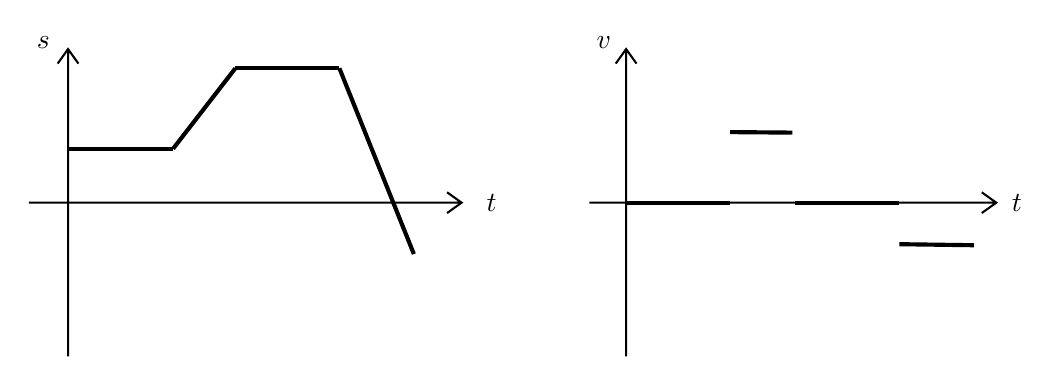
\begin{tikzpicture}[x=0.75pt,y=0.75pt,yscale=-1,xscale=1]
	%uncomment if require: \path (0,300); %set diagram left start at 0, and has height of 300

	%Shape: Axis 2D [id:dp5986556027961727]
	\draw  (51,155) -- (259.5,155)(69.88,81) -- (69.88,229) (252.5,150) -- (259.5,155) -- (252.5,160) (64.88,88) -- (69.88,81) -- (74.88,88)  ;
	%Shape: Axis 2D [id:dp5662695542333875]
	\draw  (321,155) -- (517.11,155)(338.76,81) -- (338.76,229) (510.11,150) -- (517.11,155) -- (510.11,160) (333.76,88) -- (338.76,81) -- (343.76,88)  ;
	%Straight Lines [id:da6779633587954197]
	\draw [line width=1.5]    (70.38,129) -- (120.5,129) ;
	%Straight Lines [id:da9167817945203716]
	\draw [line width=1.5]    (338.76,155) -- (388.88,155) ;
	%Straight Lines [id:da25933988363695937]
	\draw [line width=1.5]    (120.5,129) -- (150.5,90.25) ;
	%Straight Lines [id:da8168651142384409]
	\draw [line width=1.5]    (388.88,121) -- (418.88,121.25) ;
	%Straight Lines [id:da30217738665424876]
	\draw [line width=1.5]    (150.5,90.25) -- (200.62,90.25) ;
	%Straight Lines [id:da10190075508153096]
	\draw [line width=1.5]    (420.26,155) -- (470.38,155) ;
	%Straight Lines [id:da9005064343267386]
	\draw [line width=1.5]    (200.62,90.25) -- (236.5,179.75) ;
	%Straight Lines [id:da3440663507084676]
	\draw [line width=1.5]    (470.38,175) -- (506.26,175.5) ;

	% Text Node
	\draw (58,78) node    {$s$};
	% Text Node
	\draw (274,155) node    {$t$};
	% Text Node
	\draw (328,78) node    {$v$};
	% Text Node
	\draw (526.98,155) node    {$t$};

	\end{tikzpicture}
\end{figure}

In maniera del tutto analoga è possibile ottenere dal grafico della velocità l'accelerazione scalare media e istantanea.

\begin{gather}
	\boxed{a_\textup{media} (t_1, t_2)= \frac{v(t_2)-v(t_1)}{t_2 - t_1}} \\
	\boxed{a_\textup{istantanea}=a(t)=\lim_{\Delta t \to 0} \frac{\Delta v} {\Delta t} =\frac{dv}{dt}=\frac{d^2s}{dt^2}=s''(t)}
\end{gather}

Risulta evidente che se dall'ascissa curvilinea è possibile arrivare alla velocità e all'accelerazione, può essere attuato anche il procedimento inverso: ossia ricavare le legge oraria $s(t)$ nota la dipendenza dal tempo dell'accelerazione istantanea, $a(t)$. Questo problema è conosciuto come \textbf{problema inverso}.

\begin{gather*}
	a(t)=\frac{dv}{dt} \implies dv=a(t) dt \implies \int^{v(t)}_{v(t_0)} dv = \int^t_{t_0} a(t)\,dt \\
	\implies v(t)-v(t_0)=\int^t_{t_0} a(t)\,dt \implies v(t) = v(t_0)+\int^t_{t_0} a(t)\,dt
\end{gather*}

Si ha nella soluzione una costante $v(t_0)$, che rappresenta la velocità del punto all'istante $t_0$. Per calcolare esplicitamente $v(t)$ si devono conoscere la forma analitica di $a(t)$ e la velocità iniziale $v_0$.
Possiamo ora andare a ricavare l'ascissa curvilinea:

\begin{gather*}
	v(t)=\frac{ds}{dt} \implies ds=v(t) dt \implies \int^{s(t)}_{s(t_0)} ds = \int^t_{t_0} v(t)\,dt \\
	\implies s(t)=s(t_0)+\int^t_{t_0} v(t) \,dt
\end{gather*}

Il termine $s(t_0)$ rappresenta la posizione iniziale del punto, occupata nell'istante iniziale $t_0$. Pertanto per calcolare $s(t)$, nota $v(t)$, è necessario conoscere tale posizione iniziale.

Nello studio del moto di un punto materiale, si pone particolare attenzione a due specifiche tipologie di moto, quello uniforme e quello uniformemente accelerato.

Si parla di \textbf{moto uniforme} quando la legge oraria del moto è tale per cui la velocità scalare è costante nel tempo. In questo caso $a(t)=0$. Si ottiene una funzione lineare nel tempo.

\begin{gather*}
	a(t)=0 \implies v(t)=\text{costante} \\
	s(t)=s(t_0)+ \int^t_{t_0} v(t_0) \,dt \implies s(t)=s_0 + v_0 (t - t_0)
\end{gather*}

\begin{figure}[htpb]
	\centering

	\tikzset{every picture/.style={line width=0.75pt}} %set default line width to 0.75pt

	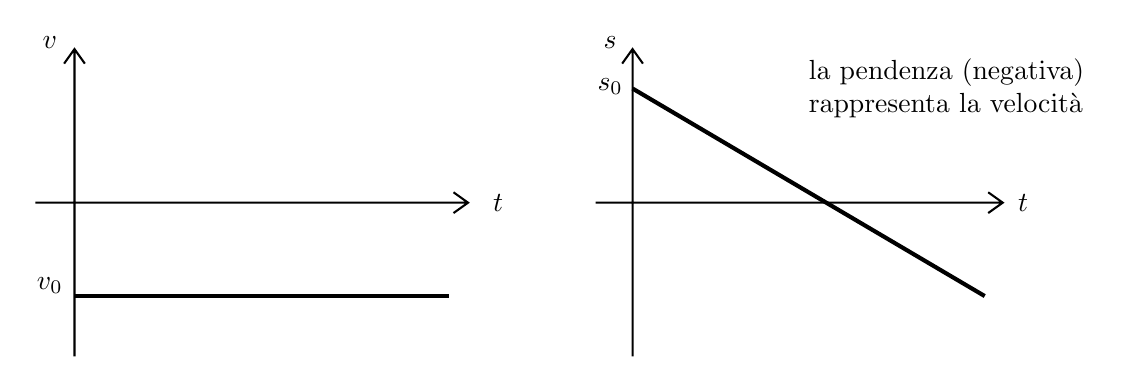
\begin{tikzpicture}[x=0.75pt,y=0.75pt,yscale=-1,xscale=1]
	%uncomment if require: \path (0,300); %set diagram left start at 0, and has height of 300

	%Shape: Axis 2D [id:dp35300894905623537]
	\draw  (51,155) -- (259.5,155)(69.88,81) -- (69.88,229) (252.5,150) -- (259.5,155) -- (252.5,160) (64.88,88) -- (69.88,81) -- (74.88,88)  ;
	%Straight Lines [id:da6687997804192232]
	\draw [line width=1.5]    (69.88,200) -- (250.27,200) ;
	%Shape: Axis 2D [id:dp10601630570504228]
	\draw  (321,155) -- (517.11,155)(338.76,81) -- (338.76,229) (510.11,150) -- (517.11,155) -- (510.11,160) (333.76,88) -- (338.76,81) -- (343.76,88)  ;
	%Straight Lines [id:da791609347568192]
	\draw [line width=1.5]    (338.76,100) -- (508.43,200) ;

	% Text Node
	\draw (58,78) node    {$v$};
	% Text Node
	\draw (274,155) node    {$t$};
	% Text Node
	\draw (58,195) node    {$v_0$};
	% Text Node
	\draw (328,78) node    {$s$};
	% Text Node
	\draw (526.98,155) node    {$t$};
	% Text Node
	\draw (328,99) node    {$s_0$};
	% Text Node
	\draw (490,100) node   [align=left] {la pendenza (negativa)\\rappresenta la velocità};

	\end{tikzpicture}
\end{figure}

Si parla di \textbf{moto uniformemente accelerato} quando la legge oraria del moto è tale per cui l'accelerazione scalare è costante nel tempo.

\[
	a(t)=a_0 \implies v(t)=v_0 + a_0 (t-t_0)
\]

\begin{figure}[htpb]
	\centering
		

	\tikzset{every picture/.style={line width=0.75pt}} %set default line width to 0.75pt

	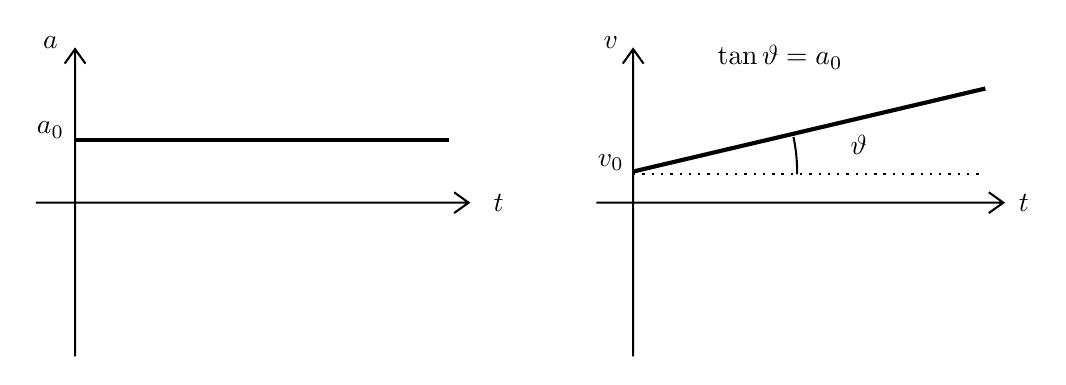
\begin{tikzpicture}[x=0.75pt,y=0.75pt,yscale=-1,xscale=1]
	%uncomment if require: \path (0,300); %set diagram left start at 0, and has height of 300

	%Shape: Axis 2D [id:dp1770714194583043]
	\draw  (51,155) -- (259.5,155)(69.88,81) -- (69.88,229) (252.5,150) -- (259.5,155) -- (252.5,160) (64.88,88) -- (69.88,81) -- (74.88,88)  ;
	%Straight Lines [id:da2762035008236656]
	\draw [line width=1.5]    (69.88,125) -- (250.27,125) ;
	%Shape: Axis 2D [id:dp3462618828150654]
	\draw  (321,155) -- (517.11,155)(338.76,81) -- (338.76,229) (510.11,150) -- (517.11,155) -- (510.11,160) (333.76,88) -- (338.76,81) -- (343.76,88)  ;
	%Straight Lines [id:da906495089646081]
	\draw [line width=1.5]    (338.76,140) -- (508.43,100) ;
	%Straight Lines [id:da5656057195303843]
	\draw [line width=0.75]  [dash pattern={on 0.84pt off 2.51pt}]  (338.76,141) -- (508.43,141) ;
	%Shape: Arc [id:dp4803004788697469]
	\draw  [draw opacity=0] (415.99,123.34) .. controls (417.14,128.71) and (417.75,134.29) .. (417.75,140) .. controls (417.75,140.45) and (417.75,140.9) .. (417.74,141.35) -- (338.76,140) -- cycle ; \draw   (415.99,123.34) .. controls (417.14,128.71) and (417.75,134.29) .. (417.75,140) .. controls (417.75,140.45) and (417.75,140.9) .. (417.74,141.35) ;

	% Text Node
	\draw (58,78) node    {$a$};
	% Text Node
	\draw (274,155) node    {$t$};
	% Text Node
	\draw (58,120) node    {$a_0$};
	% Text Node
	\draw (328,78) node    {$v$};
	% Text Node
	\draw (526.98,155) node    {$t$};
	% Text Node
	\draw (328,135.5) node    {$v_0$};
	% Text Node
	\draw (409.5,85) node    {$\tan \vartheta =a_0$};
	% Text Node
	\draw (447.5,127) node    {$\vartheta $};

	\end{tikzpicture}
\end{figure}

Si vede come l'accelerazione abbia l'effetto di aumentare linearmente la velocità.

\[
	\implies s(t)=s_0+ \int^t_{t_0} v(t)\,dt = \int^t_{t_0} a_0 + v_0 (t-t_0)\,dt
\]

Si trova allora:

\begin{equation}
	\boxed{s(t)=s_0+v_0 t+ \frac{1}{2}a_0 t^2}
\end{equation}

La legge oraria aumenta quadraticamente nel tempo.

Riportiamo in sintesi le leggi caratteristiche del moto uniformemente accelerato:

\[
	\begin{cases}
		a(t)=a_0 \\
		v(t) = v(t_0)+\int^t_{t_0} a(t)\,dt \\
		s(t)=s_0+v_0 t+ \frac{1}{2}a_0 t^2
	\end{cases}
\]

\begin{figure}[htpb]
	\centering
		

	\tikzset{every picture/.style={line width=0.75pt}} %set default line width to 0.75pt

	\begin{tikzpicture}[x=0.75pt,y=0.75pt,yscale=-1,xscale=1]
	%uncomment if require: \path (0,300); %set diagram left start at 0, and has height of 300

	%Curve Lines [id:da6971889067942005]
	\draw [line width=1.5]    (126.5,75) .. controls (231.5,295) and (313.5,298) .. (418.5,76) ;
	%Shape: Axis 2D [id:dp7960519414735971]
	\draw  (75.5,183) -- (503.5,183)(272.5,33) -- (272.5,270) (496.5,178) -- (503.5,183) -- (496.5,188) (267.5,40) -- (272.5,33) -- (277.5,40)  ;

	% Text Node
	\draw (259,33) node    {$s$};
	% Text Node
	\draw (518,183) node    {$t$};

	\end{tikzpicture}
\end{figure}

\section{Trattazione vettoriale della cinematica fisica}

I concetti di traiettoria e di legge oraria che la trattazione scalare separa, sono invece combinati in quella che prende il nome di cinematica vettoriale. Dal momento che la traiettoria di un punto in generale è una linea curva, la direzione e il verso dello spostamento sono informazioni istantanee e variano generalmente in ogni punto di essa. Non è quindi sufficiente specificare il valore numerico dello spostamento, ma occorre precisare in quale direzione e verso esso stia avvenendo. Ecco perché la trattazione vettoriale individua la posizione del punto materiale tramite un vettore posizione. Esso è definito univocamente dalle tre coordinate $x(t), y(t), z(t)$. Infatti si ha: $\vec{r}(t)=\vec{x}(t)+\vec{y}(t)+\vec{z}(t)$. Conoscere come evolve la traiettoria nello spazio equivale a conoscere le tre leggi scalari $x=x(t), y=y(t), z=z(t)$.

\begin{figure}[htpb]
	\centering
		

	\tikzset{every picture/.style={line width=0.75pt}} %set default line width to 0.75pt

	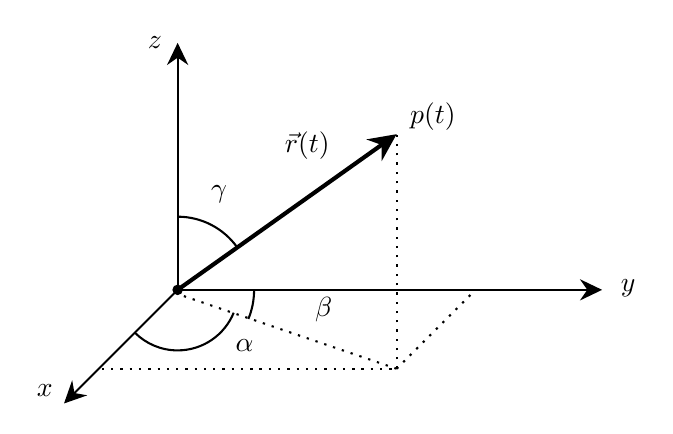
\begin{tikzpicture}[x=0.75pt,y=0.75pt,yscale=-1,xscale=1]
	%uncomment if require: \path (0,368); %set diagram left start at 0, and has height of 368

	%Straight Lines [id:da05709963918727534]
	\draw    (191,206) -- (392.5,206) ;
	\draw [shift={(395.5,206)}, rotate = 180] [fill={rgb, 255:red, 0; green, 0; blue, 0 }  ][line width=0.08]  [draw opacity=0] (10.72,-5.15) -- (0,0) -- (10.72,5.15) -- (7.12,0) -- cycle    ;
	%Straight Lines [id:da6045238370319512]
	\draw [line width=1.5]    (191,206) -- (293.24,133.32) ;
	\draw [shift={(296.5,131)}, rotate = 504.59] [fill={rgb, 255:red, 0; green, 0; blue, 0 }  ][line width=0.08]  [draw opacity=0] (13.4,-6.43) -- (0,0) -- (13.4,6.44) -- (8.9,0) -- cycle    ;
	%Straight Lines [id:da8043019054159646]
	\draw    (191,206) -- (191,90) ;
	\draw [shift={(191,87)}, rotate = 450] [fill={rgb, 255:red, 0; green, 0; blue, 0 }  ][line width=0.08]  [draw opacity=0] (10.72,-5.15) -- (0,0) -- (10.72,5.15) -- (7.12,0) -- cycle    ;
	%Straight Lines [id:da1934286126219129]
	\draw    (191,206) -- (138.37,258.63) ;
	\draw [shift={(136.25,260.75)}, rotate = 315] [fill={rgb, 255:red, 0; green, 0; blue, 0 }  ][line width=0.08]  [draw opacity=0] (10.72,-5.15) -- (0,0) -- (10.72,5.15) -- (7.12,0) -- cycle    ;
	%Straight Lines [id:da9724944386541952]
	\draw  [dash pattern={on 0.84pt off 2.51pt}]  (296.5,244) -- (296.5,131) ;
	%Straight Lines [id:da9950812379998912]
	\draw  [dash pattern={on 0.84pt off 2.51pt}]  (296.5,244) -- (334,206.5) ;
	%Straight Lines [id:da05573249238067435]
	\draw  [dash pattern={on 0.84pt off 2.51pt}]  (154.5,244) -- (296.5,244) ;
	%Shape: Circle [id:dp5872605017768655]
	\draw  [fill={rgb, 255:red, 0; green, 0; blue, 0 }  ,fill opacity=1 ] (189,206) .. controls (189,204.9) and (189.9,204) .. (191,204) .. controls (192.1,204) and (193,204.9) .. (193,206) .. controls (193,207.1) and (192.1,208) .. (191,208) .. controls (189.9,208) and (189,207.1) .. (189,206) -- cycle ;
	%Straight Lines [id:da62906602305837]
	\draw  [dash pattern={on 0.84pt off 2.51pt}]  (296.5,244) -- (191,208) ;
	%Shape: Arc [id:dp9794837241454388]
	\draw  [draw opacity=0] (190.69,170.75) .. controls (190.79,170.75) and (190.9,170.75) .. (191,170.75) .. controls (202.77,170.75) and (213.2,176.52) .. (219.6,185.39) -- (191,206) -- cycle ; \draw   (190.69,170.75) .. controls (190.79,170.75) and (190.9,170.75) .. (191,170.75) .. controls (202.77,170.75) and (213.2,176.52) .. (219.6,185.39) ;
	%Shape: Arc [id:dp49268886952965163]
	\draw  [draw opacity=0] (218.01,217.02) .. controls (213.66,227.67) and (203.21,235.17) .. (191,235.17) .. controls (183,235.17) and (175.75,231.94) .. (170.48,226.73) -- (191,206) -- cycle ; \draw   (218.01,217.02) .. controls (213.66,227.67) and (203.21,235.17) .. (191,235.17) .. controls (183,235.17) and (175.75,231.94) .. (170.48,226.73) ;
	%Shape: Arc [id:dp8952397992417833]
	\draw  [draw opacity=0] (227.83,206.57) .. controls (227.76,211.33) and (226.78,215.87) .. (225.07,220.03) -- (191,206) -- cycle ; \draw   (227.83,206.57) .. controls (227.76,211.33) and (226.78,215.87) .. (225.07,220.03) ;

	% Text Node
	\draw (253.5,136.5) node    {$\vec{r}( t)$};
	% Text Node
	\draw (127,254.5) node    {$x$};
	% Text Node
	\draw (180,87) node    {$z$};
	% Text Node
	\draw (211,160.17) node    {$\gamma $};
	% Text Node
	\draw (223.17,233) node    {$\alpha $};
	% Text Node
	\draw (261.33,215.33) node    {$\beta $};
	% Text Node
	\draw (408,205) node    {$y$};
	% Text Node
	\draw (314,122.67) node    {$p( t)$};

	\end{tikzpicture}
\end{figure}

\paragraph{Esempio:}

\[
	\vec{r}(t)=
		\begin{cases}
			x(t)=t^2+1 \\
			y(t)=4t \\
			z(t)=2
		\end{cases}
\]

Si isola $t$, eliminando la dipendenza da esso:

\[
	\begin{cases}
		t=\frac{y}{4} \\
		x=\frac{y^2}{16}+1 \\
		z=2
	\end{cases}
\]

Una volta individuata la traiettoria, bisogna capire come la posizione evolve nel tempo. A tal fine, si introduce un \textbf{vettore velocità} che è definito come la derivata del vettore posizione nel tempo.

\[
	\vec{v}(t)=\frac{d\vec{s}}{dt}
\]

Fare la derivata di un vettore significa derivare le tre funzioni scalari $x(t), y(t), z(t)$, che lo definiscono.	

\[
	\vec{v}(t)
		\begin{cases}
			v_x(t)=\frac{dx}{dt}=2t \\
			v_y(t)=\frac{dy}{dt}=4 \\
			v_z(t)=\frac{dz}{dt}=0
		\end{cases}
\]

La velocità scalare introdotta nell'ambito della trattazione scalare non è altro che la lunghezza di questo vettore velocità.

\begin{gather*}
	\norm{\vec{v}(t)}=\sqrt{v_x^2+v_y^2+v_z^2}=\sqrt{4t^2+16} \\
	s(t)=\underbrace{s(t_0)}_{=0}+\int^t_{t_0} 2\sqrt{t^2+4}\,dt
\end{gather*}

Mentre in precedenza è stata introdotta l'ascissa curvilinea per descrivere lo spostamento del punto lungo la traiettoria, la grandezza vettoriale analoga che viene ivi definita prende il nome di \textbf{raggio vettore}, o \textbf{vettore spostamento}. La sua direzione coincide con la corda che congiunge due punti considerati sulla traiettoria. Bisogna prestare molta attenzione a non confondere $\Delta\vec{r}$ con lo spazio effettivamente percorso lungo la curva, due concetti ben diversi.

\begin{figure}[htpb]
	\centering
		

	\tikzset{every picture/.style={line width=0.75pt}} %set default line width to 0.75pt

	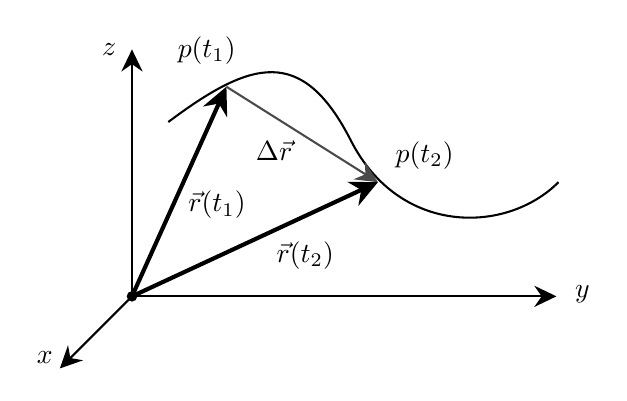
\begin{tikzpicture}[x=0.75pt,y=0.75pt,yscale=-1,xscale=1]
	%uncomment if require: \path (0,300); %set diagram left start at 0, and has height of 300

	%Straight Lines [id:da4221153943908629]
	\draw    (212,171) -- (413.5,171) ;
	\draw [shift={(416.5,171)}, rotate = 180] [fill={rgb, 255:red, 0; green, 0; blue, 0 }  ][line width=0.08]  [draw opacity=0] (10.72,-5.15) -- (0,0) -- (10.72,5.15) -- (7.12,0) -- cycle    ;
	%Straight Lines [id:da6791623240738924]
	\draw [line width=1.5]    (212,171) -- (255.86,73.65) ;
	\draw [shift={(257.5,70)}, rotate = 474.25] [fill={rgb, 255:red, 0; green, 0; blue, 0 }  ][line width=0.08]  [draw opacity=0] (13.4,-6.43) -- (0,0) -- (13.4,6.44) -- (8.9,0) -- cycle    ;
	%Straight Lines [id:da14897452664630717]
	\draw    (212,171) -- (212,55) ;
	\draw [shift={(212,52)}, rotate = 450] [fill={rgb, 255:red, 0; green, 0; blue, 0 }  ][line width=0.08]  [draw opacity=0] (10.72,-5.15) -- (0,0) -- (10.72,5.15) -- (7.12,0) -- cycle    ;
	%Straight Lines [id:da5843316458197236]
	\draw    (212,171) -- (179.37,203.63) ;
	\draw [shift={(177.25,205.75)}, rotate = 315] [fill={rgb, 255:red, 0; green, 0; blue, 0 }  ][line width=0.08]  [draw opacity=0] (10.72,-5.15) -- (0,0) -- (10.72,5.15) -- (7.12,0) -- cycle    ;
	%Shape: Circle [id:dp3769141587673239]
	\draw  [fill={rgb, 255:red, 0; green, 0; blue, 0 }  ,fill opacity=1 ] (210,171) .. controls (210,169.9) and (210.9,169) .. (212,169) .. controls (213.1,169) and (214,169.9) .. (214,171) .. controls (214,172.1) and (213.1,173) .. (212,173) .. controls (210.9,173) and (210,172.1) .. (210,171) -- cycle ;
	%Curve Lines [id:da20792216723267476]
	\draw    (229.5,87) .. controls (269.5,57) and (294,50) .. (317.5,96) .. controls (341,142) and (392.5,141) .. (417.5,116) ;
	%Straight Lines [id:da3898407246017126]
	\draw [line width=1.5]    (212,171) -- (326.87,117.68) ;
	\draw [shift={(330.5,116)}, rotate = 515.1] [fill={rgb, 255:red, 0; green, 0; blue, 0 }  ][line width=0.08]  [draw opacity=0] (13.4,-6.43) -- (0,0) -- (13.4,6.44) -- (8.9,0) -- cycle    ;
	%Straight Lines [id:da62028222338974]
	\draw [color={rgb, 255:red, 74; green, 74; blue, 74 }  ,draw opacity=1 ][line width=0.75]    (257.5,70) -- (327.96,114.4) ;
	\draw [shift={(330.5,116)}, rotate = 212.22] [fill={rgb, 255:red, 74; green, 74; blue, 74 }  ,fill opacity=1 ][line width=0.08]  [draw opacity=0] (10.72,-5.15) -- (0,0) -- (10.72,5.15) -- (7.12,0) -- cycle    ;

	% Text Node
	\draw (253,127) node    {$\vec{r}( t_1)$};
	% Text Node
	\draw (170,200.5) node    {$x$};
	% Text Node
	\draw (201,52) node    {$z$};
	% Text Node
	\draw (429,170) node    {$y$};
	% Text Node
	\draw (248,52.67) node    {$p( t_1)$};
	% Text Node
	\draw (353,103.17) node    {$p( t_2)$};
	% Text Node
	\draw (295.5,151.5) node    {$\vec{r}( t_2)$};
	% Text Node
	\draw (280.5,101) node    {$\Delta \vec{r}$};

	\end{tikzpicture}
\end{figure}

Si va ora a definire la \textbf{velocità media vettoriale} come:

\[
	\vec{v}_{\text{media}}=\frac{\Delta\vec{r}}{\Delta t}
\]
$\vec{v}_{\text{media}}$ avrà stessa direzione e verso di $\Delta\vec{r}$, l'intervallo di tempo infatti è uno scalare sempre positivo.

\[
	\vec{v}_{\text{media}}\implies \begin{cases} v_{\text{media} \,x} =\frac{\Delta x}{\Delta t} \\ v_{\text{media} \,y} =\frac{\Delta y}{\Delta t} \\ v_{\text{media} \,z} =\frac{\Delta z}{\Delta t} \end{cases}
\]

Per definire la \textbf{velocità vettoriale istantanea}, dobbiamo far tendere a $0$ l'intervallo di tempo, passaggio che equivale a ricondursi al limite del rapporto incrementale:

\[
	\vec{v}(t)=\lim_{\Delta t \to 0} \frac{\Delta \vec{r}}{\Delta t}=\frac{d\vec{r}}{dt}=\vec{r'}(t)
\]

Conoscere la velocità istantanea vettoriale significa conoscere tre funzioni che informano su come varia la velocità lungo gli assi $x, y, z$. Quando $t \to t_0$ il vettore $\Delta\vec{r}$ tende in modulo a diventare esattamente pari allo spazio percorso sulla traiettoria. In particolare l'incremento $d\vec{r}$ del raggio vettore risulta in direzione tangente alla traiettoria, per cui possiamo scrivere

\begin{equation}
	\label{velocita}
	\boxed{\vec{v}(t)=\frac{d\vec{r}}{dt}=\frac{ds}{dt}\,\vec{u}_t}
\end{equation}

dove $\vec{u}_t$ è il versore della tangente alla curva. $\vec{v}_\text{istantanea}$ infatti ha lo stesso valore della velocità scalare e stesso verso e direzione del versore intrinseco $\vec{u}_t$.
Questi ultimi due fattori sono caratteristiche intrinseche alla traiettoria, che non dipendono ovvero dalla scelta del sistema di riferimento. Ecco perché tale scrittura ~\eqref{velocita} è nota come \textit{scomposizione del vettore velocità in componenti intrinseche alla traiettoria}.
Si può spostare l'origine $O$ in un'altra posizione, si possono ruotare gli assi, ma la direzione, il verso, il modulo della velocità e la curva restano gli stessi. Si parla di invarianza delle relazioni vettoriali rispetto alla scelta del sistema di riferimento.

Definito il vettore velocità è possibile poi andare a definire un vettore accelerazione che, come al solito, sarà:

\[
	\vec{a}_{\text{media}}=\frac{\vec{v}_{t_1}-\vec{v}_{t_0}}{t_1-t_0}
\]

Riducendo gli intervalli di tempo, si otterrà la derivata del vettore velocità, che corrisponde al vettore accelerazione al generico istante $t$:

\[
	\vec{a}_{\text{ist}}=\frac{d\vec{v}}{dt} \implies
		\begin{cases}
		a_x=\frac{dv_x}{dt}=\frac{d^2s_x}{dt^2} \\
		a_y=\frac{dv_y}{dt}=\frac{d^2s_y}{dt^2}\\
		a_z=\frac{dv_z}{dt}=\frac{d^2s_z}{dt^2}
		\end{cases}
\]
$\vec{a}(t)$ è scomponibile in componenti cartesiane, che informano su come varia nel tempo le componenti in $x, y, z$ dell'accelerazione.

Si noti come fondamentalmente l'approccio della cinematica vettoriale sia quello di andare a studiare tre leggi scalari: il problema inverso si ripete tre volte. La trattazione ha un difetto perché nasconde il comportamento effettivo del moto del punto materiale. Dare una descrizione di questo tipo non permette infatti di visualizzare direttamente come esso si muove: combinare i tre moti infatti non è così semplice.

\subsection{Rappresentazione del vettore accelerazione in componenti intrinseche alla traiettoria}

Mentre il vettore velocità ha direzione tangente alla traiettoria e può quindi sempre essere espresso come:

\[
	\vec{v}(t)=\frac{ds}{dt}\,\vec{u}_t=v(t)\,\vec{u}_t \quad \text{Espressione intrinseca del vettore velocità}
\]

Il vettore accelerazione ammette una scomposizione in due componenti intrinseche alla traiettoria.

\begin{figure}[htpb]
	\centering
		

	\tikzset{every picture/.style={line width=0.75pt}} %set default line width to 0.75pt

	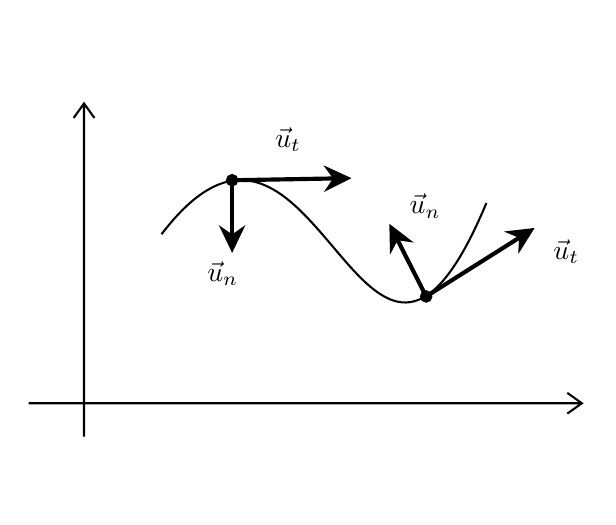
\begin{tikzpicture}[x=0.75pt,y=0.75pt,yscale=-1,xscale=1]
	%uncomment if require: \path (0,300); %set diagram left start at 0, and has height of 300

	%Shape: Axis 2D [id:dp3400766029212272]
	\draw  (82,197.45) -- (348.5,197.45)(108.65,53) -- (108.65,213.5) (341.5,192.45) -- (348.5,197.45) -- (341.5,202.45) (103.65,60) -- (108.65,53) -- (113.65,60)  ;
	%Curve Lines [id:da5974370210452586]
	\draw    (146,116) .. controls (221.5,17) and (243.5,242) .. (302.5,101) ;
	%Straight Lines [id:da8529673806643632]
	\draw [line width=1.5]    (181,90) -- (233.5,89.07) ;
	\draw [shift={(237.5,89)}, rotate = 538.99] [fill={rgb, 255:red, 0; green, 0; blue, 0 }  ][line width=0.08]  [draw opacity=0] (13.4,-6.43) -- (0,0) -- (13.4,6.44) -- (8.9,0) -- cycle    ;
	%Shape: Circle [id:dp6915133943146423]
	\draw  [fill={rgb, 255:red, 0; green, 0; blue, 0 }  ,fill opacity=1 ] (177.5,90) .. controls (177.5,88.62) and (178.62,87.5) .. (180,87.5) .. controls (181.38,87.5) and (182.5,88.62) .. (182.5,90) .. controls (182.5,91.38) and (181.38,92.5) .. (180,92.5) .. controls (178.62,92.5) and (177.5,91.38) .. (177.5,90) -- cycle ;
	%Straight Lines [id:da3714954615127908]
	\draw [line width=1.5]    (180,90) -- (180,121) ;
	\draw [shift={(180,125)}, rotate = 270] [fill={rgb, 255:red, 0; green, 0; blue, 0 }  ][line width=0.08]  [draw opacity=0] (13.4,-6.43) -- (0,0) -- (13.4,6.44) -- (8.9,0) -- cycle    ;
	%Straight Lines [id:da6433144150732559]
	\draw [line width=1.5]    (273.5,146) -- (257.56,114.57) ;
	\draw [shift={(255.75,111)}, rotate = 423.11] [fill={rgb, 255:red, 0; green, 0; blue, 0 }  ][line width=0.08]  [draw opacity=0] (13.4,-6.43) -- (0,0) -- (13.4,6.44) -- (8.9,0) -- cycle    ;
	%Straight Lines [id:da8505210239426837]
	\draw [line width=1.5]    (273.5,146) -- (322.37,115.14) ;
	\draw [shift={(325.75,113)}, rotate = 507.72] [fill={rgb, 255:red, 0; green, 0; blue, 0 }  ][line width=0.08]  [draw opacity=0] (13.4,-6.43) -- (0,0) -- (13.4,6.44) -- (8.9,0) -- cycle    ;
	%Shape: Circle [id:dp8706507040610654]
	\draw  [fill={rgb, 255:red, 0; green, 0; blue, 0 }  ,fill opacity=1 ] (271,146) .. controls (271,144.62) and (272.12,143.5) .. (273.5,143.5) .. controls (274.88,143.5) and (276,144.62) .. (276,146) .. controls (276,147.38) and (274.88,148.5) .. (273.5,148.5) .. controls (272.12,148.5) and (271,147.38) .. (271,146) -- cycle ;

	% Text Node
	\draw (175.5,135) node    {$\vec{u}_n$};
	% Text Node
	\draw (207,70.5) node    {$\vec{u}_t$};
	% Text Node
	\draw (341,124.5) node    {$\vec{u}_t$};
	% Text Node
	\draw (273,102.5) node    {$\vec{u}_n$};

	\end{tikzpicture}
\end{figure}

Data una traiettoria qualunque, è possibile definire in ogni suo punto due versori particolari: quello tangente, $\vec{u_t}$, con verso concorde a $d\vec{r}$, e quello normale (o ortogonale), $\vec{u_n}$. Esso sarà perpendicolare al vettore tangente e punterà verso l'interno della concavità della traiettoria. Questi due versori individuano un piano che prende il nome di \textbf{piano osculatore}. Essi ovviamente non mantengono direzione, ad eccezione del \emph{moto rettilineo}.
Per ottenere la scomposizione dell'accelerazione nelle due componenti, la si ridefinisce come:

\begin{equation}
	\label{eqn:scomposizione}
	\boxed{\vec{a}(t)=\frac{d\vec{v}}{dt}=\frac{d(\vec{u}_t\,v)}{dt}=\vec{u}_t\,\frac{dv}{dt}+v\,\frac{d\vec{u}_t}{dt}}
\end{equation}

II primo membro di ~\eqref{eqn:scomposizione} fornisce un'informazione legata alla variazione della velocità scalare (alla quale infatti viene applicato l'operatore derivata) ed esiste quindi solo se essa varia. Ha direzione tangente alla traiettoria e per tale motivo prende il nome di \textbf{accelerazione tangenziale}. È evidente che non è pari al modulo dell'accelerazione vettoriale per via del secondo componente comparso derivando il prodotto. In esso l'operatore derivata è applicato al versore tangente $\vec{u}_t$. Il fatto che stia variando nel tempo è indice di un cambiamento di direzione sulla traiettoria. Ogni volta che quest'ultima è curvilinea esiste il secondo termine nella somma. Calcoliamolo in maniera più esplicita.

\paragraph{Derivata di un versore} Si può dimostrare che la derivata di un versore dà luogo a un vettore che ha direzione ortogonale al versore di partenza.

\[
	\vec{u}_t\cdot\vec{u}_t=1 \implies \frac{d\vec{u}_t}{dt}\cdot \vec{u}_t+ \vec{u}_t\cdot \frac{d\vec{u}_t}{dt}=0
\]

Il prodotto scalare gode della proprietà commutativa, perciò i due termini ottenuti tramite la derivata del prodotto sono uguali. Segue allora che:

\[
	2\vec{u}_t\cdot\frac{d\vec{u}_t}{dt}=0 \implies \vec{u}_t\perp \frac{d\vec{u}_t}{dt} \implies \frac{d\vec{u}_t}{dt} \parallel \vec{u}_n
\]

La variazione angolare $d\vartheta$ si può ricondurre alle grandezze cinematiche che sono state introdotte, essendo legata alla variazione infinitesima di ascissa curvilinea:

\[
	ds=\rho\,d\vartheta
\]

In particolare, l'angolo $d\vartheta$ individuato dai due versori, è equivalente all'angolo individuato nel cerchio di raggio unitario rappresentato in figura.

\[
	\norm{d\vec{u}_t}=1\,d\vartheta
\]

Fatta questa premessa, è possibile affermare che:

\[
	\frac{d\vec{u}_t}{dt}=\frac{d\vartheta}{dt}\,\vec{u}_n
\]

e, di conseguenza:

\[
	v\,\frac{d\vec{u}_t}{dt}= v\,\frac{d\vartheta}{dt}\,\vec{u}_n=\frac{v}{\rho}\,\frac{ds}{dt}\,\vec{u}_n=\frac{v^2}{\rho}\,\vec{u}_n
\]

\begin{equation}
	\boxed{\vec{a}_n=\frac{v^2}{\rho}\,\vec{u}_n}
\end{equation}

Il fatto che all'aumentare della curvatura il raggio del cerchio osculatore diminuisca, porta a definire la \textbf{curvatura} della traiettoria come il reciproco di tale raggio:

\[
	k:=\frac{1}{\rho}
\]

si ha allora:

\[
	\vec{a}_n=k\,{v^2}\,\vec{u}_n
\]

\begin{figure}[htb!]
	\vspace*{-50mm}
	\centering

	\tikzset{every picture/.style={line width=0.75pt}} %set default line width to 0.75pt

	\begin{tikzpicture}[x=0.75pt,y=0.75pt,yscale=-1,xscale=1]
	%uncomment if require: \path (0,225); %set diagram left start at 0, and has height of 225

	%Shape: Circle [id:dp5208500816458348]
	\draw   (127.5,128) .. controls (127.5,78.57) and (167.57,38.5) .. (217,38.5) .. controls (266.43,38.5) and (306.5,78.57) .. (306.5,128) .. controls (306.5,177.43) and (266.43,217.5) .. (217,217.5) .. controls (167.57,217.5) and (127.5,177.43) .. (127.5,128) -- cycle ;
	%Curve Lines [id:da09806334628889624]
	\draw    (67,149) .. controls (320.5,-168) and (308.5,325) .. (457.5,40) ;
	%Straight Lines [id:da6623793670478895]
	\draw  [dash pattern={on 0.84pt off 2.51pt}]  (217,38.5) -- (217,128) ;
	%Straight Lines [id:da9470005639819916]
	\draw  [dash pattern={on 0.84pt off 2.51pt}]  (278.33,61.92) -- (217,128) ;
	%Shape: Arc [id:dp21315146015323272]
	\draw  [draw opacity=0] (217.37,90.67) .. controls (226.82,90.76) and (235.43,94.36) .. (241.96,100.23) -- (217,128) -- cycle ; \draw   (217.37,90.67) .. controls (226.82,90.76) and (235.43,94.36) .. (241.96,100.23) ;
	%Straight Lines [id:da09170287984211711]
	\draw [line width=1.5]    (217,38.5) -- (290.38,38.5) ;
	\draw [shift={(294.38,38.5)}, rotate = 180] [fill={rgb, 255:red, 0; green, 0; blue, 0 }  ][line width=0.08]  [draw opacity=0] (13.4,-6.43) -- (0,0) -- (13.4,6.44) -- (8.9,0) -- cycle    ;
	%Straight Lines [id:da8134422742349374]
	\draw [line width=1.5]    (278.33,61.92) -- (325.89,104.34) ;
	\draw [shift={(328.88,107)}, rotate = 221.73] [fill={rgb, 255:red, 0; green, 0; blue, 0 }  ][line width=0.08]  [draw opacity=0] (13.4,-6.43) -- (0,0) -- (13.4,6.44) -- (8.9,0) -- cycle    ;

	% Text Node
	\draw (206.67,71) node    {$\rho $};
	% Text Node
	\draw (214.67,138.33) node    {$C$};
	% Text Node
	\draw (236,78.33) node    {$d\vartheta $};
	% Text Node
	\draw (252.5,19.33) node    {$\vec{u}_t( t_1)$};
	% Text Node
	\draw (341,69.83) node    {$\vec{u}_t( t_1 +dt)$};
	% Text Node
	\draw (375,156.83) node    {$ds\ =\rho \ d\vartheta $};

	\end{tikzpicture}
	\vspace*{-30mm}
\end{figure}

Quindi il raggio di curvatura compare al denominatore perché comunica il fatto che l'accelerazione normale aumenta tanto più la curvatura è elevata. Ovviamente il valore dell'accelerazione normale dipende anche dal quadrato della velocità. Quando la traiettoria è rettilinea, l'accelerazione normale è pari a zero e $\rho$ tende a infinito, quindi il vettore accelerazione coincide con il vettore accelerazione tangenziale.

\subsection{Esempi di moto}

Questa sezione si concentra su alcune particolari tipologie di moto che ricorrono con frequenza.

\subsubsection{Moto parabolico}

Il moto parabolico è quello caratteristico di corpi pesanti che si muovono in prossimità della superficie terrestre, soggetti alla sola accelerazione di gravità. In questo ambito si trascura l'eventuale attrito creato dall'aria.
Nella descrizione di tale moto, è preferibile utilizzare un riferimento cartesiano in cui una delle due direzioni è parallela a $\vec{g}$. Si tratta di un moto piano poiché la velocità sta sempre sul piano individuato dai vettori costanti $\vec{v}_0$ e $\vec{g}$. Dal momento che ciò che è noto è l'accelerazione lungo le due componenti ($\vec{g}$ lungo le $y$ e nulla lungo le $x$) il problema si riduce alla risoluzione di due problemi inversi.

\begin{figure}[htpb]
	\centering
		

	\tikzset{every picture/.style={line width=0.75pt}} %set default line width to 0.75pt

	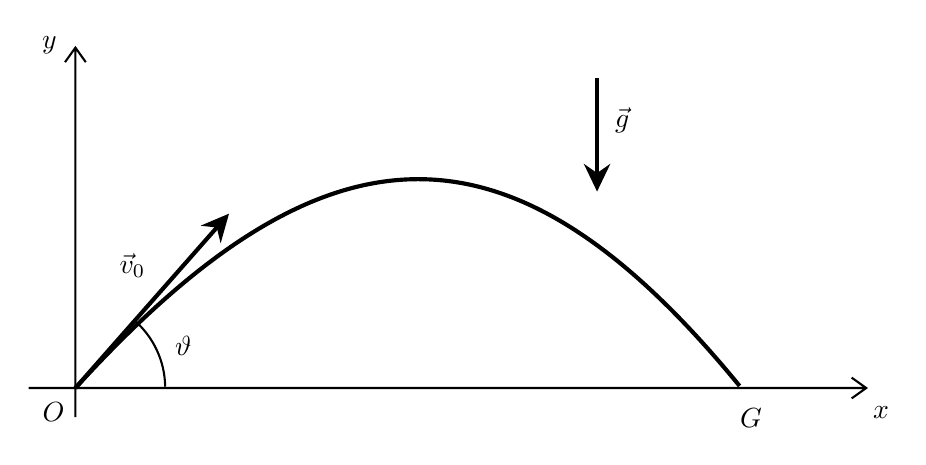
\begin{tikzpicture}[x=0.75pt,y=0.75pt,yscale=-1,xscale=1]
	%uncomment if require: \path (0,300); %set diagram left start at 0, and has height of 300

	%Shape: Axis 2D [id:dp21763212568332824]
	\draw  (70,217) -- (473.5,217)(92.5,53) -- (92.5,231) (466.5,212) -- (473.5,217) -- (466.5,222) (87.5,60) -- (92.5,53) -- (97.5,60)  ;
	%Straight Lines [id:da05203031601857888]
	\draw [line width=1.5]    (92.5,217) -- (163.86,136) ;
	\draw [shift={(166.5,133)}, rotate = 491.38] [fill={rgb, 255:red, 0; green, 0; blue, 0 }  ][line width=0.08]  [draw opacity=0] (13.4,-6.43) -- (0,0) -- (13.4,6.44) -- (8.9,0) -- cycle    ;
	%Straight Lines [id:da509522474347498]
	\draw [line width=1.5]    (343.83,67.67) -- (343.83,118.33) ;
	\draw [shift={(343.83,122.33)}, rotate = 270] [fill={rgb, 255:red, 0; green, 0; blue, 0 }  ][line width=0.08]  [draw opacity=0] (13.4,-6.43) -- (0,0) -- (13.4,6.44) -- (8.9,0) -- cycle    ;
	%Shape: Arc [id:dp904536839291062]
	\draw  [draw opacity=0] (120.98,184.45) .. controls (129.89,192.25) and (135.56,203.65) .. (135.75,216.37) -- (92.5,217) -- cycle ; \draw   (120.98,184.45) .. controls (129.89,192.25) and (135.56,203.65) .. (135.75,216.37) ;
	%Curve Lines [id:da9850378824791992]
	\draw [line width=1.5]    (92.5,217) .. controls (214.5,83) and (303.5,83) .. (412.5,216) ;

	% Text Node
	\draw (80,52) node    {$y$};
	% Text Node
	\draw (82,228.67) node    {$O$};
	% Text Node
	\draw (418,231.33) node    {$G$};
	% Text Node
	\draw (480.67,228.67) node    {$x$};
	% Text Node
	\draw (120,158) node    {$\vec{v}_0$};
	% Text Node
	\draw (356,88) node    {$\vec{g}$};
	% Text Node
	\draw (144.5,196.5) node    {$\vartheta $};

	\end{tikzpicture}
	\vspace*{-10mm}
\end{figure}

\[
	\begin{cases}
		a_x=0 \\
		a_y=-g
	\end{cases}
\]

Sono necessarie le condizioni iniziali del punto:

\[
	\vec{r}(t_0=0)= \begin{cases} x(t_0)=0 \\ y(t_0)=0 \end{cases} \vec{v}(t_0)=\begin{cases} v_{0x}=v_0\cos\vartheta \\ v_{0y}=v_0\sin\vartheta \end{cases}
\]
È possibile quindi ricavare le leggi orarie dei moti proiettati, che sono:

\begin{gather*}
	\vec{v}(t) =
		\begin{cases}
			v_x(t)=v_0\cos\vartheta+\int a_0(x)\,dt=v_0\cos\vartheta \\
			v_y(t)=v_0\sin\vartheta+\int (-g)\,dt=v_0\sin\vartheta-gt
		\end{cases} \\
	\vec{r}(t) =
		\begin{cases}
			x(t)=x_0+\int v_x\,dt=v_0\cos\vartheta\,t \quad \text{moto uniforme} \\
			y(t)=y_0+\int v_y\,dt=v_0\sin\vartheta\,t-\frac{1}{2}gt^2 \quad \text{moto unif. accelerato}
		\end{cases}
\end{gather*}

Il moto parabolico è la composizione di un moto uniforme lungo l'asse orizzontale, uniformemente accelerato lungo l'asse ortogonale. La traiettoria è quella di una parabola. Calcoliamo $y(x)$ per poterla visualizzare:

\[
	t=\frac{x(t)}{v_0\cos\vartheta} \implies y(x)=\tan\vartheta x-\frac{g}{2} \,\frac{x^2}{v_0^2\,\cos^2\vartheta}
\]

La traiettoria infatti viene sempre ricavata eliminando il tempo tra $x(t)$ e $y(t)$ e ottenendo così la funzione $y(x)$, che è l'equazione di una parabola. La distanza orizzontale fra il punto di partenza e quello di arrivo è detta \textbf{gittata del lancio}. Per calcolarla si impone $y(x)=0$ e si ottiene:

\begin{gather*}
	y=v_0\sin\vartheta t-\frac{1}{2}gt^2=0 \implies v_0\sin\vartheta-\frac{1}{2}gt=0 \implies t=\frac{2v_0\sin\vartheta}{g} \\
	x_G=v_{0x}t=\underbrace{v_0\cos\vartheta}_{v_{0x}}\,\underbrace{\frac{2v_0\sin\vartheta}{g}}_{t}=2x_M \quad \text{per la simmetria della parabola}
\end{gather*}

Conoscendo $x_M$ è anche possibile calcolare l'ascissa del punto di massima altezza raggiunta, che è, pertanto:

\begin{align*}
	y(x_M)&=\tan\vartheta\,\frac{v_0^2\cos\vartheta \sin\vartheta}{g}-\frac{g}{2}\,\left(\frac{v_0^2\cos\vartheta \sin\vartheta}{g}\right)^2\,\frac{1}{v_0^2\cos^2\vartheta} \\
	y(x_M)&=\frac{v_0^2 \sin^2\vartheta}{g}-\frac{v_0^2}{2g}\,\sin^2\vartheta=\frac{v_0^2\sin^2\vartheta}{2g}
\end{align*}

L'altezza massima raggiunta nel moto parabolico può essere calcolata anche in altri modi, ad esempio imponendo $y'(x)=0$, oppure considerando il fatto che la componente verticale della velocità è nulla al vertice della parabola e che quindi in tale istante $v_x(t)=0$. Il tempo totale di volo è pari al tempo impiegato a percorre $OG$ con velocità costante $v(x)=v(t_0 )\cos\vartheta$. Evidentemente questo tempo è pari al tempo necessario per salire all'altezza $y_{\text{max}}$ e ritornare al suolo. Notiamo infine che nella posizione $G$ la velocità è la stessa in modulo che alla partenza, ma è posta simmetricamente rispetto all'asse $x$. Si noti come le caratteristiche geometriche del moto parabolico di un corpo vicino alla superficie terrestre possano effettivamente essere comprese in modo semplice nel sistema cartesiano adottato, che è in definitiva il più naturale per questo problema in cui vi è una direzione di particolare importanza, quella di $\vec{g}$, a 90 gradi con una direzione di uso pratico molto comune, quella orizzontale.

\subsubsection{Moto rettilineo}

Il moto rettilineo si svolge lungo una retta sulla quale vengono fissati arbitrariamente un'origine e un verso (asse $x$). Il moto del punto è descrivibile tramite una sola coordinata $x(t)$.

\subsubsection{Moto circolare}

Si chiama moto circolare un moto piano la cui traiettoria è rappresentata da una circonferenza.\\

\begin{figure}[htpb]
	\centering
	\tikzset{every picture/.style={line width=0.75pt}} %set default line width to 0.75pt

	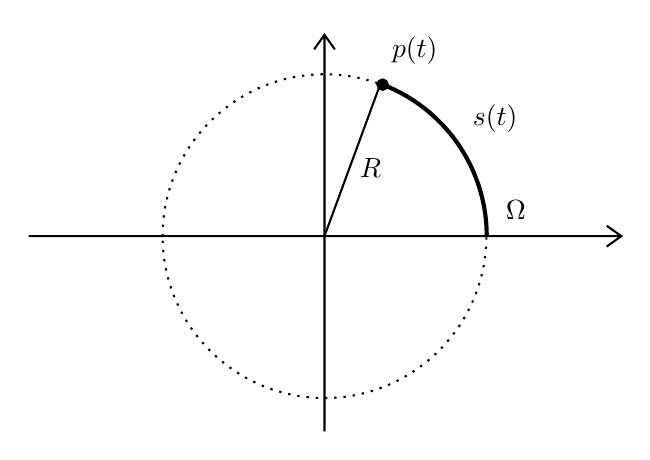
\begin{tikzpicture}[x=0.75pt,y=0.75pt,yscale=-1,xscale=1]
	%uncomment if require: \path (0,300); %set diagram left start at 0, and has height of 300

	%Shape: Axis 2D [id:dp6452357499911294]
	\draw  (50,161) -- (335.5,161)(192.5,64) -- (192.5,255) (328.5,156) -- (335.5,161) -- (328.5,166) (187.5,71) -- (192.5,64) -- (197.5,71)  ;
	%Shape: Circle [id:dp4813437894170338]
	\draw  [dash pattern={on 0.84pt off 2.51pt}] (114.5,161) .. controls (114.5,117.92) and (149.42,83) .. (192.5,83) .. controls (235.58,83) and (270.5,117.92) .. (270.5,161) .. controls (270.5,204.08) and (235.58,239) .. (192.5,239) .. controls (149.42,239) and (114.5,204.08) .. (114.5,161) -- cycle ;
	%Shape: Arc [id:dp7325164530727912]
	\draw  [draw opacity=0][line width=1.5]  (219.45,87.6) .. controls (249.15,98.51) and (270.4,126.94) .. (270.66,160.37) -- (192.5,161) -- cycle ; \draw  [line width=1.5]  (219.45,87.6) .. controls (249.15,98.51) and (270.4,126.94) .. (270.66,160.37) ;
	%Shape: Circle [id:dp743830313409608]
	\draw  [fill={rgb, 255:red, 0; green, 0; blue, 0 }  ,fill opacity=1 ] (218,88) .. controls (218,86.62) and (219.12,85.5) .. (220.5,85.5) .. controls (221.88,85.5) and (223,86.62) .. (223,88) .. controls (223,89.38) and (221.88,90.5) .. (220.5,90.5) .. controls (219.12,90.5) and (218,89.38) .. (218,88) -- cycle ;
	%Straight Lines [id:da3632039280212016]
	\draw    (219.45,87.6) -- (192.5,161) ;

	% Text Node
	\draw (284.67,148.33) node    {$\Omega $};
	% Text Node
	\draw (274.67,104.33) node    {$s( t)$};
	% Text Node
	\draw (236,71.67) node    {$p( t)$};
	% Text Node
	\draw (214.67,128.33) node    {$R$};

	\end{tikzpicture}
\end{figure}

Il moto circolare può essere descritto facendo riferimento allo spazio percorso sulla circonferenza $s(t)$ oppure utilizzando l'angolo $\vartheta(t)$ sotteso dall'arco $s(t)$, con $\vartheta (t)=\frac{s(t)}{R}$. L'assumere come variabile l'angolo $\vartheta(t)$ significa in pratica porsi in un sistema di coordinate polari di centro $O$ in cui il moto avviene con raggio di curvatura $\norm{\vec{r}(t)}=R=\text{costante}$ e $\vartheta (t)$ variabile. Si è naturalmente interessati alle variazioni dell'angolo nel tempo e pertanto definiamo la \textbf{velocità angolare} come la derivata dell'angolo rispetto al tempo:

\begin{gather*}
	\omega=\frac{d\vartheta}{dt}=\frac{ds}{dt}\,\frac{1}{R}=\frac{v}{R}\\
	1 \text{ rad}=\frac{s}{R} \qquad \text{angolo quando $s=R$}
\end{gather*}

Risulta che la velocità angolare è proporzionale alla velocità con cui è descritta la circonferenza, se $v$ è variabile, anche $\omega$ lo è.

\[
	\Gamma=
	\begin{cases}
		(x-x_0)^2+(y-y_0)^2=R^2 \\
		z=z_0
	\end{cases}
\]

Il moto circolare più semplice è quello \emph{uniforme}, $v$ e $\omega$ sono costanti e le leggi orarie, con riferimento alle due variabili utilizzate, si scrivono:

\[
	s(t)=s_0+vt \quad \vartheta(t)=\vartheta_0+\int^t_{t_0} \omega\,dt
\]

Il moto circolare uniforme è un moto accelerato con accelerazione costante, ortogonale alla traiettoria:

\[
	a=a_n=\frac{v^2}{R}=\omega^2 R
\]

Nel caso del moto circolare \emph{non uniforme}, oltre all'accelerazione centripeta, che è variabile perché la velocità varia in modulo, bisogna considerare anche l'accelerazione tangenziale $a = \frac{dv}{dt}$. Siccome è variabile $\omega$, si definisce l'\textbf{accelerazione angolare}:

\begin{gather*}
	\alpha(t)=\frac{d\omega}{dt}=\frac{dv}{dt}\,\frac{1}{R}= \frac{a(t)}{R} \\
	d\omega=\alpha(t) \,dt \implies \int^{\omega(t)}_{\omega(t_0)} d\omega=\int^t_{t_0} \alpha(t)\,dt \\
	\omega(t)=\omega(t_0)+\int^t_{t_0}\alpha(t)\,dt \\
	d\vartheta=\omega\,dt \implies \int^{\vartheta(t)}_{\vartheta(t_0)} d\vartheta =\int^t_{t_0}\omega\,dt \\
\end{gather*}

\begin{equation}
	\boxed{\vartheta(t)=\vartheta(t_0)+\omega_0(t-t_0)+\frac{1}{2}\alpha_0(t-t_0)^2}
\end{equation}

\subsubsection{Moto armonico}

La descrizione di tale moto è affrontata in dettaglio nel capitolo 5.

\section{Cinematica relativa}

Quando il sistema di riferimento in generale si muove di moto qualunque, è necessario sottoporre le leggi affrontate finora ad alcune modifiche. Sperimentalmente è provato che le leggi fisiche non dipendono dalla scelta del sistema di riferimento. Fissato questo e stabilita una certa proprietà, essa resta vera anche se cambiano l'origine e l'orientamento degli assi coordinati, ovvero se ci si riferisce ad un altro sistema ottenuto con una rotazione, una traslazione o con un'operazione combinata. Non esiste pertanto un punto di riferimento privilegiato dello spazio e nemmeno un'orientazione privilegiata: lo spazio appare omogeneo e isotropo. La caratteristica sostanziale di invarianza acquista un aspetto formale se le leggi fisiche vengono espresse come relazione tra entità che godono anch'esse delle suddette proprietà di invarianza, come le grandezze scalari o quelle vettoriali.

La situazione si presenta diversa quando un fenomeno viene osservato da due sistemi di riferimento in moto l'uno rispetto all'altro, poiché in tal caso non sussiste invarianza delle leggi fisiche e lo spostamento viene descritto in modi differenti.

L'osservatore finora considerato è sempre stato posto in un \emph{sistema di riferimento assoluto}, dato cioè da un'origine fissa nello spazio e da tre direzioni preferenziali. Tuttavia si possono presentare situazioni in cui l'osservatore è in movimento. Si definisce in tali casi un sistema di riferimento mobile che si identifica sempre come un sistema di riferimento cartesiano. Esso tuttavia può:

\begin{itemize}
	\item \emph{traslare} nello spazio con una velocità di traslazione. Si ricordi che una traslazione nello spazio è un movimento rigido attraverso il quale i tre versori che identificano il sistema di riferimento non ruotano mai (non è necessariamente un moto lungo la traiettoria rettilinea).
	\item \emph{ruotare} nello spazio con una certa velocità angolare.
\end{itemize}

L'obbiettivo della cinematica relativa è quello di studiare il moto del punto materiale rispetto all'osservatore fisso e quello mobile e trovare delle relazioni che permettono di passare facilmente dall'una all'altra descrizione del fenomeno.

\begin{figure}[htpb]
	\centering
	
	\tikzset{every picture/.style={line width=0.75pt}} %set default line width to 0.75pt

	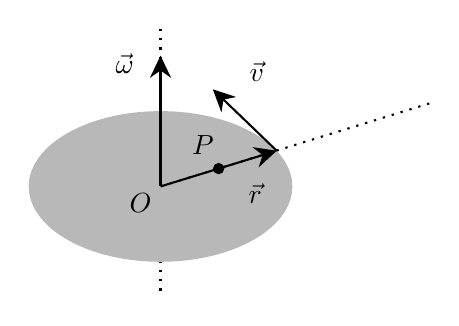
\begin{tikzpicture}[x=0.75pt,y=0.75pt,yscale=-1,xscale=1]
	%uncomment if require: \path (0,300); %set diagram left start at 0, and has height of 300

	%Straight Lines [id:da9471165549419143]
	\draw  [dash pattern={on 0.84pt off 2.51pt}]  (214,77) -- (214,206) ;
	%Shape: Ellipse [id:dp6549012336948079]
	\draw  [draw opacity=0][fill={rgb, 255:red, 184; green, 184; blue, 184 }  ,fill opacity=1 ] (150.5,153) .. controls (150.5,132.96) and (178.93,116.71) .. (214,116.71) .. controls (249.07,116.71) and (277.5,132.96) .. (277.5,153) .. controls (277.5,173.04) and (249.07,189.29) .. (214,189.29) .. controls (178.93,189.29) and (150.5,173.04) .. (150.5,153) -- cycle ;
	%Straight Lines [id:da2622224811431515]
	\draw    (214,93) -- (214,153) ;
	\draw [shift={(214,90)}, rotate = 90] [fill={rgb, 255:red, 0; green, 0; blue, 0 }  ][line width=0.08]  [draw opacity=0] (10.72,-5.15) -- (0,0) -- (10.72,5.15) -- (7.12,0) -- cycle    ;
	%Straight Lines [id:da23746773885354222]
	\draw  [dash pattern={on 0.84pt off 2.51pt}]  (343.5,113) -- (214,153) ;
	%Straight Lines [id:da5943734544225967]
	\draw    (241.36,108.28) -- (270,135.8) ;
	\draw [shift={(239.2,106.2)}, rotate = 43.86] [fill={rgb, 255:red, 0; green, 0; blue, 0 }  ][line width=0.08]  [draw opacity=0] (10.72,-5.15) -- (0,0) -- (10.72,5.15) -- (7.12,0) -- cycle    ;
	%Straight Lines [id:da7598081460438388]
	\draw    (267.13,136.68) -- (214,153) ;
	\draw [shift={(270,135.8)}, rotate = 162.93] [fill={rgb, 255:red, 0; green, 0; blue, 0 }  ][line width=0.08]  [draw opacity=0] (10.72,-5.15) -- (0,0) -- (10.72,5.15) -- (7.12,0) -- cycle    ;
	%Shape: Circle [id:dp006380434010266001]
	\draw  [fill={rgb, 255:red, 0; green, 0; blue, 0 }  ,fill opacity=1 ] (239.8,144.4) .. controls (239.8,143.18) and (240.78,142.2) .. (242,142.2) .. controls (243.22,142.2) and (244.2,143.18) .. (244.2,144.4) .. controls (244.2,145.62) and (243.22,146.6) .. (242,146.6) .. controls (240.78,146.6) and (239.8,145.62) .. (239.8,144.4) -- cycle ;

	% Text Node
	\draw (196.8,93.6) node    {$\vec{\omega }$};
	% Text Node
	\draw (259.6,156.4) node    {$\vec{r}$};
	% Text Node
	\draw (260.4,97.6) node    {$\vec{v}$};
	% Text Node
	\draw (204.4,160.8) node    {$O$};
	% Text Node
	\draw (234.4,133.2) node    {$P$};

	\end{tikzpicture}
\end{figure}

Per definire un oggetto che ruota era stata introdotta precedentemente la variazione angolare e ad essa erano state associate una velocità e un'accelerazione angolari: quantità scalari.

\[
	v=\omega r \qquad a_t=\alpha r \qquad a_n=\omega^2 r=\frac{v^2}{r}
\]

Queste informazioni possono essere espresse anche in termini vettoriali. Si definisce \textbf{vettore velocità angolare} $\vec{\omega}$ con le seguenti proprietà: il modulo è $\omega=\frac{d\vartheta}{dt}$, la direzione è perpendicolare al piano in cui avviene il moto e il verso è tale per cui dall'estremo del vettore $\vec{\omega}$ il moto appaia antiorario. Si ha:

\[
	\vec{v}=\vec{\omega} \times \vec{r}
\]

Si tratta di una relazione completa che lega la velocità (sempre tangente) al vettore velocità angolare. Di norma, si pensa $\vec{\omega}$ applicato nel centro della circonferenza. La formula soprastante resta comunque valida se $\vec{\omega}$ è applicato in un qualsiasi altro punto dell'asse di rotazione, la cui direzione è individuata da $\vec{u}_z$. Noto $\vec{\omega}$, sono individuati pertanto l'asse di rotazione, il piano del moto, il verso con cui è percorsa la circonferenza e come varia l'angolo nel tempo.

\[
	\vec{\omega}=\omega\, \vec{u}_z
\]

Tutti i punti del disco possiedono un'unica velocità angolare definita come in figura. Da $\vec{\omega}$, per derivazione rispetto al tempo, si ottiene il \textbf{vettore accelerazione angolare} $\vec{\alpha}$ che risulta parallelo a $\vec{\omega}$ (dato che questo ha direzione costante) verso determinato dalla variazione del modulo di $\vec{\omega}$ e modulo $\alpha=\frac{d\omega}{dt}$.

\[
	\vec{\alpha}=\alpha \vec{u}_z
\]

Essa si esprime come segue:

\[
	\vec{a}=\frac{d\vec{v}}{dt}=\frac{d(\vec{\omega} \times \vec{r})}{dt}=\frac{d\vec{\omega}}{dt} \times \vec{r}+\vec{\omega} \times \frac{d\vec{r}}{dt}=\underbrace{\vec{\alpha} \times \vec{r}}_{\vec{a_t}}\, + \underbrace{\vec{\omega} \times \vec{v}}_{\vec{a_n}}
\]

Da questa relazione si vede che il vettore accelerazione tangente è pari al prodotto vettoriale fra l'accelerazione angolare e il raggio della circonferenza su cui si sta muovendo il punto. L'accelerazione normale è invece frutto di un doppio prodotto vettoriale:

\[
	\vec{a}_n=\vec{\omega} \times \vec{v}=\vec{\omega} \times ( \vec{r} \times \vec{\omega})
\]

Si noti che che $\vec{\omega}$ e $\vec{r}$ sono ortogonali, quindi è sufficiente moltiplicare i loro moduli. Il risultato $\vec{\omega} \times \vec{r}$ è un vettore tangente alla circonferenza che va moltiplicato per $\vec{\omega}$, ortogonale al piano. Il vettore risultante è dunque ortogonale a quella tangente e a $\vec{u}_z$, puntante verso l'asse di rotazione. Il suo modulo è semplicemente il prodotto dei moduli, perché entra sempre in gioco $\sin\frac{\pi}{2}$.

Si supponga di avere un disco che ruota su sé stesso. Tutti i suoi punti si muovono con la stessa velocità angolare, perché devono compiere nello stesso tempo un giro, essendo un corpo che ruota rigidamente, senza deformarsi. Tuttavia tali punti non hanno tutti la stessa velocità $\vec{v}$ perché, scritto scalarmente, $v=\omega r$, quindi essi avranno velocità maggiore man mano che ci si sposta verso l'esterno. In generale quindi si ha stessa velocità angolare ma velocità lineari differenti. Analogo discorso si applica per l'accelerazione tangente e per quella normale.

\section{Legge di composizione delle velocità}

L'osservatore fisso identifica la posizione del punto $P$ tramite il vettore posizione $\vec{r}_{\text{ass}}$, scomponibile in coordinate cartesiane come segue:

\[
	\vec{r}(t)=x(t) \vec{u}_x+y(t)\vec{u}_y+z(t)\vec{u}_z
\]

Nel corso del tempo $x(t)$ cambia, ma i tre versori rimangono invariati perché il sistema di riferimento è fermo nello spazio.

\begin{figure}[htpb]
	\centering

	\tikzset{every picture/.style={line width=0.75pt}} %set default line width to 0.75pt

	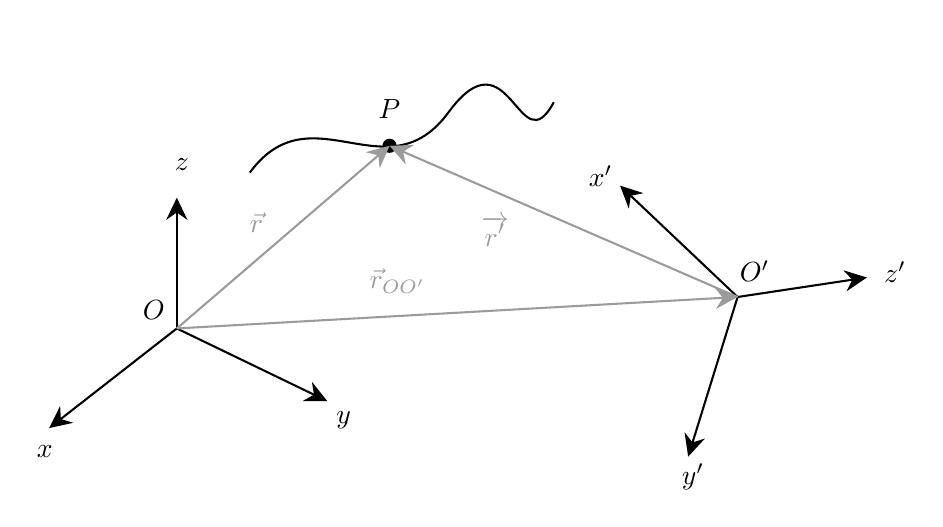
\begin{tikzpicture}[x=0.75pt,y=0.75pt,yscale=-1,xscale=1]
	%uncomment if require: \path (0,300); %set diagram left start at 0, and has height of 300

	%Straight Lines [id:da25086700744423784]
	\draw    (108,133) -- (108,193) ;
	\draw [shift={(108,130)}, rotate = 90] [fill={rgb, 255:red, 0; green, 0; blue, 0 }  ][line width=0.08]  [draw opacity=0] (10.72,-5.15) -- (0,0) -- (10.72,5.15) -- (7.12,0) -- cycle    ;
	%Straight Lines [id:da19724660264049287]
	\draw    (48.86,239.15) -- (108,193) ;
	\draw [shift={(46.5,241)}, rotate = 322.03] [fill={rgb, 255:red, 0; green, 0; blue, 0 }  ][line width=0.08]  [draw opacity=0] (10.72,-5.15) -- (0,0) -- (10.72,5.15) -- (7.12,0) -- cycle    ;
	%Straight Lines [id:da7967137770227075]
	\draw    (177.8,226.7) -- (108,193) ;
	\draw [shift={(180.5,228)}, rotate = 205.77] [fill={rgb, 255:red, 0; green, 0; blue, 0 }  ][line width=0.08]  [draw opacity=0] (10.72,-5.15) -- (0,0) -- (10.72,5.15) -- (7.12,0) -- cycle    ;
	%Straight Lines [id:da6556661966529236]
	\draw    (437.51,168.9) -- (378.18,177.85) ;
	\draw [shift={(440.47,168.46)}, rotate = 171.43] [fill={rgb, 255:red, 0; green, 0; blue, 0 }  ][line width=0.08]  [draw opacity=0] (10.72,-5.15) -- (0,0) -- (10.72,5.15) -- (7.12,0) -- cycle    ;
	%Straight Lines [id:da9702780467154479]
	\draw    (323.73,126.25) -- (378.18,177.85) ;
	\draw [shift={(321.55,124.19)}, rotate = 43.46] [fill={rgb, 255:red, 0; green, 0; blue, 0 }  ][line width=0.08]  [draw opacity=0] (10.72,-5.15) -- (0,0) -- (10.72,5.15) -- (7.12,0) -- cycle    ;
	%Straight Lines [id:da16665976731656107]
	\draw    (355.26,251.89) -- (378.18,177.85) ;
	\draw [shift={(354.37,254.75)}, rotate = 287.2] [fill={rgb, 255:red, 0; green, 0; blue, 0 }  ][line width=0.08]  [draw opacity=0] (10.72,-5.15) -- (0,0) -- (10.72,5.15) -- (7.12,0) -- cycle    ;
	%Straight Lines [id:da8237388779050301]
	\draw [color={rgb, 255:red, 155; green, 155; blue, 155 }  ,draw opacity=1 ]   (108,193) -- (375.18,178.01) ;
	\draw [shift={(378.18,177.85)}, rotate = 536.79] [fill={rgb, 255:red, 155; green, 155; blue, 155 }  ,fill opacity=1 ][line width=0.08]  [draw opacity=0] (10.72,-5.15) -- (0,0) -- (10.72,5.15) -- (7.12,0) -- cycle    ;
	%Shape: Boxed Bezier Curve [id:dp8912748108905522]
	\draw    (143.18,117.91) .. controls (172.76,77.6) and (209.3,129.22) .. (238.88,88.9) .. controls (268.46,48.59) and (272.96,115.15) .. (289.63,83.97) ;
	%Shape: Circle [id:dp9836014349883189]
	\draw  [fill={rgb, 255:red, 0; green, 0; blue, 0 }  ,fill opacity=1 ] (207.6,105) .. controls (207.6,103.4) and (208.9,102.1) .. (210.5,102.1) .. controls (212.1,102.1) and (213.4,103.4) .. (213.4,105) .. controls (213.4,106.6) and (212.1,107.9) .. (210.5,107.9) .. controls (208.9,107.9) and (207.6,106.6) .. (207.6,105) -- cycle ;
	%Straight Lines [id:da2664802092852583]
	\draw [color={rgb, 255:red, 155; green, 155; blue, 155 }  ,draw opacity=1 ]   (108,193) -- (208.22,106.95) ;
	\draw [shift={(210.5,105)}, rotate = 499.35] [fill={rgb, 255:red, 155; green, 155; blue, 155 }  ,fill opacity=1 ][line width=0.08]  [draw opacity=0] (10.72,-5.15) -- (0,0) -- (10.72,5.15) -- (7.12,0) -- cycle    ;
	%Straight Lines [id:da46149717327452744]
	\draw [color={rgb, 255:red, 155; green, 155; blue, 155 }  ,draw opacity=1 ]   (378.18,177.85) -- (213.25,106.2) ;
	\draw [shift={(210.5,105)}, rotate = 383.48] [fill={rgb, 255:red, 155; green, 155; blue, 155 }  ,fill opacity=1 ][line width=0.08]  [draw opacity=0] (10.72,-5.15) -- (0,0) -- (10.72,5.15) -- (7.12,0) -- cycle    ;

	% Text Node
	\draw (44.4,252.2) node    {$x$};
	% Text Node
	\draw (188.4,237.2) node    {$y$};
	% Text Node
	\draw (110.4,114.2) node    {$z$};
	% Text Node
	\draw (312.24,119.53) node    {$x'$};
	% Text Node
	\draw (356.66,264.44) node    {$y'$};
	% Text Node
	\draw (454.06,165.69) node    {$z'$};
	% Text Node
	\draw (210.4,87.2) node    {$P$};
	% Text Node
	\draw (96.9,184.2) node    {$O$};
	% Text Node
	\draw (386.4,165.2) node    {$O'$};
	% Text Node
	\draw (146.4,142.2) node  [color={rgb, 255:red, 155; green, 155; blue, 155 }  ,opacity=1 ]  {$\vec{r}$};
	% Text Node
	\draw (261.4,146.2) node  [color={rgb, 255:red, 155; green, 155; blue, 155 }  ,opacity=1 ]  {$\overrightarrow{r'}$};
	% Text Node
	\draw (214.4,170.2) node  [color={rgb, 255:red, 155; green, 155; blue, 155 }  ,opacity=1 ]  {$\vec{r}_{OO'}$};

	\end{tikzpicture}
\end{figure}

L'osservatore relativo descrive il moto del punto $P$ definendo un vettore posizione $\vec{r'}(t)$ che identifica la posizione di $P$ dal sistema di riferimento $Oxy'$. Anche $\vec{r'}(t)$ può essere scomposto in componenti cartesiane rispetto al sistema di riferimento relativo. Otterremo:

\[
	\vec{r'}(t)=x'(t) \vec{u}_{x'}+y'(t)\vec{u}_{y'}+z'(t)\vec{u}_{z'}
\]

La differenza è che in questa espressione di vettore di posizione, oltre alle coordinate del punto materiale, anche i versori $\vec{u}_{x'}$, $\vec{u}_{y'}$, $\vec{u}_{z'}$ variano nel tempo nel momento in cui il sistema ruota (se esso invece subisce la sola traslazione ciò non accade).

Successivamente, si definisce un terzo versore che congiunge il sistema di riferimento fisso con il sistema di riferimento mobile che viene indicato come $\vec{r}_{oo'}$. Esso individua la posizione dell'origine del sistema di riferimento mobile rispetto al sistema di riferimento fisso, rappresenta quindi le coordinate di $O'$ rispetto ai versori $\vec{u}_x, \vec{u}_y, \vec{u}_z$.

\[
	\vec{r}_{oo'}(t)=x_{oo'}(t)\vec{u}_x+y_{oo'}(t)\vec{u}_y+z_{oo'}(t)\vec{u}_z
\]

Definiti questi tre vettori è possibile osservare che vi è una relazione semplice che li lega:

\begin{equation}
	\label{relativo}
	\boxed{\vec{r}(t)=\vec{r'}(t)+\vec{r}_{oo'}(t)}
\end{equation}

Derivando membro a membro si ottiene l'informazione che fornisce il legame fra le velocità. La velocità del punto $P$ rispetto al sistema fisso, che viene chiamata \emph{velocità assoluta}, è data da:

\[
	\vec{v}=\frac{d\vec{r}}{dt}= \frac{dx}{dt}\vec{u}_x + \frac{dy}{dt}\vec{u}_y + \frac{dz}{dt}\vec{u}_z
\]

Derivando il vettore posizione $\vec{r'}$ si ottiene:

\[
	\frac{d\vec{r'}}{dt}=\underbrace{\frac{dx'}{dt}\vec{u}_{x'}+\frac{dy'}{dt}\vec{u}_{y'}+\frac{dz'}{dt}\vec{u}_{z'}}_A+ \underbrace{x'(t) \frac{d\vec{u}_{x'}}{dt}+ y'(t) \frac{d\vec{u}_{y'}}{dt}+ z'(t) \frac{d\vec{u}_{z'}}{dt}}_B
\]

Il termine $A$ rappresenta la velocità del punto $P$ misurata dal sistema di riferimento mobile, viene chiamata \emph{velocità relativa}. Il termine $B$ nasce invece quando i versori variano direzione nel tempo, ossia quando il sistema di riferimento relativo ruota.

\paragraph{Formula di Poisson} La derivata di un versore che varia nel tempo, è un vettore ortogonale a quello di partenza, il cui modulo dà informazione su quanto rapidamente varia la sua direzione nel tempo. Si ha:

\[
	\frac{d\vec{u}_x}{dt}=\vec{\omega} \times \vec{u}_x
\]

Dove $\vec{\omega}$ è la velocità angolare con cui ruota il versore.

I tre versori sono rigidamente legati l'uno all'altro, nel senso che le loro mutue orientazioni non possono cambiare: alla rotazione di uno, con velocità angolare $\omega$, corrisponde la rotazione degli altri due con la stessa velocità angolare, come se essi fossero parte di un unico corpo indeformabile. Si ottiene quindi:

\begin{equation*}
	\begin{aligned}
		\frac{d\vec{r'}}{dt} &= \frac{dx'}{dt} \vec{u}_{x'}+x'(t)(\vec{\omega} \times \vec{u}_{x'})+\frac{dy'}{dt} \vec{u}_{y'} +y'(t)(\vec{\omega} \times \vec{u}_{y'})+\frac{dz'}{dt} \vec{u}_{z'} +z'(t)(\vec{\omega} \times \vec{u}_{z'} ) \\
		&= \frac{dx'}{dt}\vec{u}_{x'}+ \frac{dy'}{dt}\vec{u}_{y'}+ \frac{dz'}{dt}\vec{u}_{z'} + \underbrace{\vec{\omega} \times (x'(t)\vec{u}_{x'}+y'(t)\vec{u}_{y'}+z'(t)\vec{u}_{z'})}_{\vec{\omega} \times \vec{r'}}
	\end{aligned}
\end{equation*}

La velocità di $O'$ rispetto al sistema di riferimento fisso, quindi la velocità di traslazione del sistema di riferimento mobile, è data da:

\[
	\frac{d\vec{r}_{oo'}}{dt}=\frac{dx_{oo'}}{dt}\vec{u}_x+\frac{dy_{oo'}}{dt}\vec{u}_y+\frac{dz_{oo'}}{dt}\vec{u}_z=\vec{v}_{oo'}
\]

In sintesi derivando la ~\eqref{relativo} si ottiene:

\[
	\vec{v}_{\text{ass}}(t)=\vec{v}_{\text{rel}}+\underbrace{(\vec{\omega} \times \vec{r'}+\vec{v}_{oo'})}_{\text{velocità di trascinamento}}=\vec{v}_{\text{rel}}+ \vec{v}_{ \text{trasc} }
\]

I termini evidenziati prendono il nome di \emph{velocità di trascinamento} del punto $P$ e rappresentano la velocità del sistema con cui è trascinato a muoversi quando lo si immagina solidale ad esso. Se il punto $P$ fosse fermo rispetto al sistema di riferimento mobile, la sua velocità misurata dal sistema fisso coinciderebbe con tale velocità, data dalla somma di un termine traslatorio con velocità istantanea $v_{oo'}$ e di un termine relativo con velocità angolare $\vec{\omega}$, variabile in generale sia in modulo che in direzione.

In forma compatta, la legge di composizione delle velocità afferma che un punto materiale in movimento rispetto ad un osservatore relativo, avrà rispetto a un osservatore fisso una velocità assoluta frutto della somma delle velocità relativa e di trascinamento.

\[
	\text{Teorema delle velocità relative} \quad \boxed{\vec{v}_{\text{ass}}=\vec{v}_{\text{rel}}+\vec{v}_{\text{trasc}}}
\]

\paragraph{Esempio} La Terra è un sistema di riferimento mobile nel tempo. In termini di velocità vettoriale si identifica come in figura. Allora un osservatore che si trova in un punto della Terra, a causa della rotazione terrestre è trascinato a ruotare insieme ad essa. La velocità angolare è costante, quella lineare è sempre più piccola verso i poli. Si tratta di un classico esempio in cui si è trascinati insieme al sistema di riferimento in cui ci si muove.

\begin{figure}[htpb]
	\centering

	\tikzset{every picture/.style={line width=0.75pt}} %set default line width to 0.75pt

	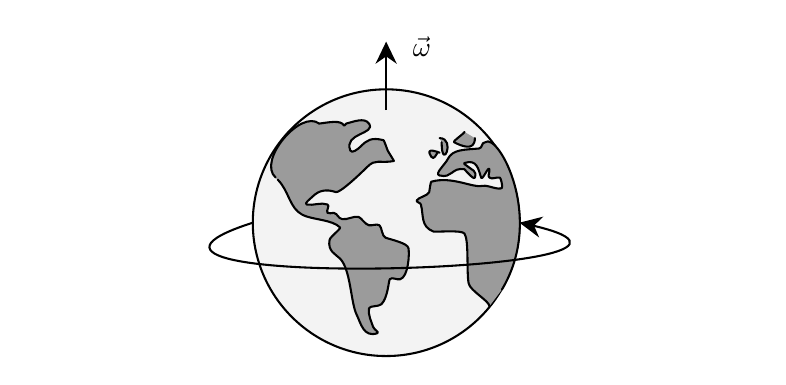
\begin{tikzpicture}[x=0.75pt,y=0.75pt,yscale=-1,xscale=1]
	%uncomment if require: \path (0,314); %set diagram left start at 0, and has height of 314

	%Shape: Circle [id:dp8683221589787924]
	\draw  [fill={rgb, 255:red, 243; green, 243; blue, 243 }  ,fill opacity=1 ] (200.5,181.75) .. controls (200.5,146.27) and (229.27,117.5) .. (264.75,117.5) .. controls (300.23,117.5) and (329,146.27) .. (329,181.75) .. controls (329,217.23) and (300.23,246) .. (264.75,246) .. controls (229.27,246) and (200.5,217.23) .. (200.5,181.75) -- cycle ;
	%Curve Lines [id:da531178027916203]
	\draw [color={rgb, 255:red, 0; green, 0; blue, 0 }  ][fill={rgb, 255:red, 155; green, 155; blue, 155 }  ,fill opacity=1 ][line width=0.75] [line join = round][line cap = round]   (212.5,161) .. controls (218.08,166.58) and (218.08,174.79) .. (224.5,178) .. controls (229.22,180.36) and (238.71,180.21) .. (242.5,184) .. controls (243.17,184.67) and (237.81,188.44) .. (237.5,190) .. controls (236.4,195.51) and (240.63,197.13) .. (242.5,199) .. controls (247.69,204.19) and (247.7,220.4) .. (250.5,226) .. controls (252.55,230.09) and (253.78,237.24) .. (260.5,235) .. controls (261.64,234.62) and (258.88,233.14) .. (258.5,232) .. controls (257.82,229.97) and (255.81,225.76) .. (256.5,223) .. controls (256.84,221.63) and (261.17,222.33) .. (262.5,221) .. controls (265.6,217.9) and (265.93,209.68) .. (266.5,209) .. controls (267.57,207.72) and (269.9,209.46) .. (271.5,209) .. controls (275.42,207.88) and (276.07,196.85) .. (275.5,194) .. controls (275.03,191.63) and (267.53,190.01) .. (264.5,189) .. controls (262.62,188.37) and (262.71,183.72) .. (261.5,183) .. controls (260.07,182.14) and (258.14,183.27) .. (256.5,183) .. controls (254.64,182.69) and (252.74,179.31) .. (251.5,179) .. controls (248.89,178.35) and (246.14,180.53) .. (243.5,180) .. controls (241.41,179.58) and (241.58,177.52) .. (239.5,177) .. controls (238.53,176.76) and (237.1,177.8) .. (236.5,177) .. controls (235.7,175.93) and (237.74,173.5) .. (236.5,173) .. controls (233.41,171.76) and (229.77,173.65) .. (226.5,173) .. controls (224.87,172.67) and (228.32,170.18) .. (229.5,169) .. controls (232.24,166.26) and (235.77,165.42) .. (240.5,167) .. controls (242.31,167.6) and (251.68,158.82) .. (255.5,155) .. controls (259.94,150.56) and (261.4,153.42) .. (268.5,152) .. controls (268.58,151.98) and (265.6,147.25) .. (265.5,147) .. controls (265.29,146.48) and (263.74,142.06) .. (263.5,142) .. controls (257.62,140.53) and (255.55,141.95) .. (252.5,145) .. controls (251.23,146.27) and (248.17,148.67) .. (247.5,147) .. controls (244.05,138.39) and (259.97,139.21) .. (256.5,134) .. controls (254.38,130.82) and (248.78,133.18) .. (245.5,134) .. controls (245.04,134.11) and (244.71,135.42) .. (244.5,135) .. controls (243.04,132.09) and (237.16,133.42) .. (232.5,134) .. controls (223.5,127) and (202.5,152) .. (211.5,160) ;
	%Curve Lines [id:da11031845277788]
	\draw [color={rgb, 255:red, 0; green, 0; blue, 0 }  ][fill={rgb, 255:red, 155; green, 155; blue, 155 }  ,fill opacity=1 ][line width=0.75] [line join = round][line cap = round]   (314.5,222) .. controls (314.5,219.46) and (305.21,214.56) .. (304.5,211) .. controls (303.43,205.66) and (304.7,190.3) .. (302.5,187) .. controls (301.23,185.09) and (288.47,186.39) .. (287.5,186) .. controls (281.32,183.53) and (282.9,178.59) .. (281.5,173) .. controls (281.27,172.09) and (279.08,171.84) .. (279.5,171) .. controls (280.25,169.5) and (284.9,168.81) .. (285.5,167) .. controls (285.57,166.79) and (286.12,162.11) .. (286.5,162) .. controls (296.58,159.12) and (306.56,165.24) .. (311.5,164) .. controls (313.49,163.5) and (318.85,166.24) .. (320.5,165) .. controls (321.07,164.57) and (320,160.1) .. (319.5,160) .. controls (317.87,159.67) and (315.8,161.04) .. (314.5,160) .. controls (313.46,159.17) and (314.82,157.29) .. (314.5,156) .. controls (314.04,154.17) and (311.1,161.79) .. (310.5,160) .. controls (309.16,155.99) and (308.58,150.97) .. (302.5,153) .. controls (301.61,153.3) and (303.83,154.33) .. (304.5,155) .. controls (305.71,156.21) and (308.65,156.54) .. (307.5,160) .. controls (307.01,161.46) and (302.51,156) .. (302.5,156) .. controls (296.19,154.95) and (296.67,160.54) .. (290.5,159) .. controls (287.77,158.32) and (293.07,153.86) .. (294.5,151) .. controls (296.84,146.33) and (302.37,146.65) .. (309.5,146) .. controls (311.28,145.84) and (310.49,143) .. (312.5,143) .. controls (318.5,138) and (341.5,179) .. (320.5,214) ;
	%Curve Lines [id:da8940953037558799]
	\draw [color={rgb, 255:red, 0; green, 0; blue, 0 }  ][fill={rgb, 255:red, 155; green, 155; blue, 155 }  ,fill opacity=1 ][line width=0.75] [line join = round][line cap = round]   (302.5,138) .. controls (302.5,138.69) and (296.61,142.55) .. (297.5,143) .. controls (300.69,144.6) and (307.5,147.77) .. (307.5,141) ;
	%Curve Lines [id:da5286705701496102]
	\draw [color={rgb, 255:red, 0; green, 0; blue, 0 }  ][fill={rgb, 255:red, 155; green, 155; blue, 155 }  ,fill opacity=1 ][line width=0.75] [line join = round][line cap = round]   (291.5,143) .. controls (291.5,157.74) and (298.55,141) .. (290.5,141) ;
	%Curve Lines [id:da1567416553514649]
	\draw [color={rgb, 255:red, 0; green, 0; blue, 0 }  ][fill={rgb, 255:red, 155; green, 155; blue, 155 }  ,fill opacity=1 ][line width=0.75] [line join = round][line cap = round]   (289.5,148) .. controls (289.09,148.41) and (287.78,151.92) .. (286.5,150) .. controls (283,144.75) and (290.27,148) .. (290.5,148) ;
	%Curve Lines [id:da02198661372958144]
	\draw    (200.5,181.75) .. controls (92.54,216.33) and (443.46,205.61) .. (330.73,182.11) ;
	\draw [shift={(329,181.75)}, rotate = 371.38] [fill={rgb, 255:red, 0; green, 0; blue, 0 }  ][line width=0.08]  [draw opacity=0] (10.72,-5.15) -- (0,0) -- (10.72,5.15) -- (7.12,0) -- cycle    ;
	%Straight Lines [id:da37712678869520455]
	\draw    (264.75,127.5) -- (264.75,97.5) ;
	\draw [shift={(264.75,94.5)}, rotate = 450] [fill={rgb, 255:red, 0; green, 0; blue, 0 }  ][line width=0.08]  [draw opacity=0] (10.72,-5.15) -- (0,0) -- (10.72,5.15) -- (7.12,0) -- cycle    ;

	% Text Node
	\draw (282,97) node    {$\vec{\omega }$};

	\end{tikzpicture}
\end{figure}

\section{Legge di composizione delle accelerazioni}

È possibile ora ricavare il legame fra le accelerazioni. Rispetto al sistema fisso l'accelerazione assoluta è data da:

\begin{gather*}
	\frac{d\vec{v}_{\text{ass} }}{dt}=\frac{d}{dt}\left(\frac{dx}{dt} \vec{u}_x + \frac{dy}{dt} \vec{u}_y+ \frac{dz}{dt} \vec{u}_z\right)=\frac{d^2x}{dt^2} \vec{u}_x+ \frac{d^2y}{dt^2} \vec{u}_y+\frac{d^2z}{dt^2} \vec{u}_z=\vec{a}_{\text{ass}} (t) \\
	\vec{a}_{\text{ass}}(t)=\frac{d\vec{v}_{\text{rel}}}{dt}+\frac{d}{dt}(\vec{\omega} \times \vec{r}_{\text{rel}})+\frac{d\vec{v}_{oo'}}{dt}
\end{gather*}

Derivando il primo termine si ha:

\[
	\frac{d\vec{v}_{\text{rel}}}{dt}=\frac{d}{dt}\left(\frac{dx'}{dt}\vec{u}_{x'}+\frac{dy'}{dt}\vec{u}_{y'}+\frac{dz'}{dt}\vec{u}_{z'}\right)=\frac{d^2x'}{dt^2} \vec{u}_{x'} + \frac{d^2y'}{dt^2} \vec{u}_{y'}+ \frac{d^2z'}{dt^2} \vec{u}_{z'}
\]

Il termine ottenuto prende il nome di \emph{accelerazione relativa}. Per quanto riguarda il secondo e il terzo termine avremo:

\begin{gather*}
	\frac{d}{dt}(\vec{\omega} \times \vec{r}_{\text{rel}})=\frac{d\vec{\omega}}{dt} \times \vec{r}_{\text{rel}}+\vec{\omega} \times \frac{d\vec{r}_{\text{rel}} }{dt} = \vec{\alpha} \times \vec{r}_{\text{rel}}+\vec{\omega} \times( \vec{v}_{\text{rel}}+\vec{\omega} \times \vec{v}_{\text{rel}}) \\
	\frac{d\vec{v}_{oo'}}{dt}= \frac{d^2x_{oo'}}{dt^2} \vec{u}_x+ \frac{d^2y_{oo'}}{dt^2} \vec{u}_y+ \frac{d^2z_{oo'}}{dt^2} \vec{u}_z=\vec{a}_{oo'}
\end{gather*}

E quindi:

\[
	\vec{a}_{\text{ass}}(t)=\vec{a}_{\text{rel}} +\vec{\omega} \times \vec{v}_{\text{rel}}+\vec{\alpha}\times \vec{r}_{\text{rel}}+\vec{\omega} \times \vec{v}_{\text{rel}}+ \vec{\omega}\times({\vec{\omega}}\times \vec{r}_{\text{rel}})+\vec{a}_{oo'}
\]

\begin{equation}
	\boxed{\vec{a}_{\text{ass}}(t)=\vec{a}_{\text{rel}} +2\,\vec{\omega} \times \vec{v}_{\text{rel}}+\vec{\alpha}\times \vec{r}_{\text{rel}}+ \vec{\omega}\times({\vec{\omega}}\times \vec{r}_{\text{rel}})+\vec{a}_{oo'}}
\end{equation}

Questo risultato è noto come \emph{legge di composizione delle accelerazioni in cinematica relativa}. Il termine:

\[
	\vec{a}_{\text{trasc}}=\underbrace{\vec{\alpha}\times \vec{r}_{\text{rel}}}_A+ \underbrace{\vec{\omega}\times({\vec{\omega}}\times \vec{r}_{\text{rel}})}_B+\vec{a}_{oo'}
\]

prende il nome di \textbf{accelerazione di trascinamento}, e rappresenta l'accelerazione con cui è portato a muoversi il punto $P$ immaginato come congelato nel sistema di riferimento mobile. Il termine:

\[
	\vec{a}_c= 2\,\vec{\omega} \times \vec{v}_{\text{rel}}
\]

prende il nome di \textbf{accelerazione di Coriolis}.
Fondamentalmente quando un punto materiale si muove in un sistema di riferimento mobile, l'accelerazione osservata da un osservatore fermo nello spazio è data dall'accelerazione percepita nel sistema di riferimento relativo, più il termine accelerazione di trascinamento.
I termini $A$ e $B$ sono le due componenti dell'accelerazione che assume il punto $P$ quando il sistema di riferimento mobile ruota. La prima è l'accelerazione normale, la seconda è l'accelerazione tangente. $\vec{a}_{oo'}$ invece è il termine legato alla traslazione del sistema mobile.
Per quanto riguarda l'accelerazione di Coriolis invece, essa esiste se e solo se il sistema di riferimento sta ruotando e il punto materiale ha una certa velocità relativa rispetto ad esso. In generale questa accelerazione esiste ad esempio quando si considera un oggetto che si muove da sud verso nord sulla Terra, che ruota su se stessa. L'effetto che si percepisce è una deviazione verso destra di tale corpo. Allo stesso effetto sono soggetti i venti sulla Terra, che deviano verso est o ad esempio le maree.
